\documentclass[10pt]{beamer}
\usetheme{metropolis}
\usecolortheme{default}

\usepackage{booktabs}
\usepackage{amsmath}
\usepackage{graphicx}
\usepackage{tikz}
\usetikzlibrary{arrows.meta, positioning}
\usepackage{multirow}

\title{The Median Voter Theorem}
\subtitle{ECO1028 - Politics Without Romance}
\author{Beatriz Gietner\\
\texttt{beatriz.gietner@dcu.ie}}
\date{\today}

\begin{document}

\maketitle

\begin{frame}{Outline}
\tableofcontents
\end{frame}


\section{Introduction \& Motivation}

\begin{frame}{Before We Begin: A Diagnostic Question}
\textbf{Quick poll - think about Irish politics:}


On a left-right economic scale (1 = far left, 10 = far right):
\begin{itemize}
\item Where would you place Fianna Fáil?
\item Where would you place Fine Gael?
\item Where would you place yourself?
\end{itemize}



\alert{Common complaint:} "I can't tell the difference between FF and FG!"



\textbf{Today's question:} Is this convergence a bug or a feature of democracy?
\end{frame}

\begin{frame}{The Central Puzzle: Why Do Parties Converge?}
\href{http://www.nytimes.com/2010/02/07/business/economy/07view.html}{\alert{\textbf{Tyler Cowen (2010):} "In Politics, Sometimes the Middle Way Really Is the Best"}}


\begin{quote}
"Economists approach political competition with a simple but potent hypothesis called the 'median voter theorem."'
\end{quote}



\begin{quote}
"Essentially, the idea is this: Any politician who strays too far from voters at the philosophical center will soon be out of office."
\end{quote}



\alert{Core insight:} There is a dynamic that pushes politicians to embrace the preferences of the typical or "median" voter, who sits squarely in the middle of public opinion.
\end{frame}

\begin{frame}{The Intuition}
\textbf{From Cowen's article:}


\begin{quote}
"A significant move to either the left or the right would open the door for a rival to take a more moderate stance, win the next election and change the agenda."
\end{quote}



\begin{quote}
"Politicians will respond to this dynamic, whether they are power-seeking demagogues or more benevolent types who use elected office to help the world."
\end{quote}



\alert{Key implication:} Centrist convergence isn't (necessarily) evidence of lack of choice - it's a \textit{prediction} of democratic competition!
\end{frame}

\begin{frame}{What You Need to Know}
\textbf{Four prerequisite pillars for understanding MVT:}

\begin{enumerate}
\item \textbf{Single-Peaked Preferences}
\begin{itemize}
\item Each voter has an ideal point on a policy dimension
\item Utility declines as you move away from that ideal
\end{itemize}


\item \textbf{Majority Rule}
\begin{itemize}
\item Decisions made by simple majority vote
\item 50\% + 1 determines the outcome
\end{itemize}


\item \textbf{Two-Party/Candidate Competition}
\begin{itemize}
\item Two main alternatives compete for votes
\item Winner-take-all system
\end{itemize}


\item \textbf{Rational Voters \& Politicians}
\begin{itemize}
\item Voters choose preferred alternative
\item Politicians maximize probability of winning
\end{itemize}
\end{enumerate}
\end{frame}

\begin{frame}{Diagnostic Check}
\textbf{Test your understanding:}

\textbf{Question 1:} Can you think of political issues where Irish voters have single-peaked preferences? (i.e., everyone has an ideal point and prefers outcomes closer to that ideal)

\textbf{Question 2:} Can you think of issues where preferences are \textit{not} single-peaked? (i.e., people might have multiple preferred options).

\textbf{Question 3:} In PR-STV (Irish electoral system), is it really "winner-take-all"?
\begin{itemize}
\item \alert{Insight:} PR-STV violates the "two-party" assumption, but government formation acts as a \textbf{"second stage."}
\item To form a coalition (50\% + 1), parties must still satisfy the median TD (and arguably the median voter).
\end{itemize}
\end{frame}

\begin{frame}{Historical Context}
\begin{columns}
\begin{column}{0.48\textwidth}
\textbf{Before Downs (1957)}
\begin{itemize}
\item Political science studied institutions, history, norms
\item Economics studied markets
\item Separate intellectual worlds
\item Little formal theory of voting
\end{itemize}
\end{column}


\begin{column}{0.48\textwidth}
\textbf{After Downs (1957)}
\begin{itemize}
\item Economic tools applied to politics
\item Formal models of electoral competition
\item Testable predictions
\item Birth of Public Choice
\end{itemize}
\end{column}
\end{columns}



\textbf{Key predecessors:}
\begin{itemize}
\item \textbf{Knut Wicksell (1896):} Unanimity and "just taxation"
\item \textbf{Duncan Black (1948):} First statement of median voter theorem
\item \textbf{Kenneth Arrow (1951):} Impossibility theorem (Nobel 1972)
\end{itemize}
\end{frame}

\begin{frame}{Anthony Downs (1957)}
\textbf{\textit{An Economic Theory of Democracy}}


\textbf{Revolutionary insights:}
\begin{itemize}
\item Parties are like firms competing for votes (analogous to profits)
\item Voters are like consumers choosing products
\item Political competition has predictable patterns
\item \alert{Parties converge to the median voter position}
\end{itemize}



\textbf{Why revolutionary?}
\begin{itemize}
\item Before: Politics was about ideals, public interest, civic duty
\item After: Politics is about strategic behaviour and incentives
\item Same logic that explains markets can explain democracy
\end{itemize}



\small{Note: Duncan Black (1948) formalized the theorem first, but Downs popularized it and explored its implications for electoral competition}
\end{frame}

\begin{frame}[allowframebreaks]{The Restaurant Illustration: Setup}
\textbf{A simple example to build intuition:}


Al, Bob, and Charlie need to pick a restaurant for lunch. They'll use majority rule.


\textbf{Preferences:}
\begin{itemize}
\item \textbf{Al} prefers cheap: \alert{\$5.00} lunch
\item \textbf{Bob} prefers moderate: \alert{\$10.00} lunch  
\item \textbf{Charlie} prefers expensive: \alert{\$20.00} lunch
\end{itemize}

\framebreak
\begin{center}
\includegraphics[width=0.85\textwidth]{restaurant_choice.png}
\end{center}




\textbf{Assumption:} Each person prefers restaurants closer in price to their ideal point.
\begin{itemize}
\item If Al must choose between \$10 and \$20, he picks \$10 (closer to \$5)
\item If Charlie must choose between \$5 and \$10, he picks \$10 (closer to \$20)
\end{itemize}



\alert{Key observation:} Bob is the \textbf{median voter}
\begin{itemize}
\item 1 person prefers cheaper (\$5)
\item 1 person prefers more expensive (\$20)
\item Bob is in the middle (\$10)
\end{itemize}
\end{frame}

\begin{frame}{The Restaurant Illustration: Voting Outcomes}
\textbf{What happens under majority rule?}


\begin{table}
\centering
\begin{tabular}{lcccc}
\toprule
\textbf{Options} & \textbf{Al} & \textbf{Bob} & \textbf{Charlie} & \textbf{Result} \\
\midrule
\$20 vs. \$5 & \$5 & \$5 & \$20 & \alert{\$5 wins (2-1)} \\

\$10 vs. \$20 & \$10 & \$10 & \$20 & \alert{\$10 wins (2-1)} \\

\$10 vs. \$5 & \$5 & \$10 & \$10 & \alert{\$10 wins (2-1)} \\
\bottomrule
\end{tabular}
\end{table}



\textbf{Pattern:}
\begin{itemize}
\item Bob (median voter) \alert{always votes for the winner}
\item \$10 (median preference) \alert{beats any alternative} in pairwise vote
\item Once we're at \$10, no other option can defeat it
\end{itemize}



This is the \textbf{weak form} of the median voter theorem: the median voter is always in the winning coalition.
\end{frame}

\begin{frame}{Weak Form vs. Strong Form}
\textbf{Weak Form:}
\begin{itemize}
\item The median voter always casts his or her vote for the policy that is adopted
\item The median voter's preference always beats any alternative in a head-to-head vote
\item Once median voter's preferred outcome is reached, it cannot be defeated in pairwise majoritarian election
\end{itemize}



\textbf{Strong Form:}
\begin{itemize}
\item The median voter always gets \alert{exactly} their most preferred policy
\item Requires additional conditions (credible commitment, perfect information)
\item This is what Downs (1957) emphasized in electoral competition
\end{itemize}



\alert{Critical distinction:} Weak form is about voting power. Strong form is about policy outcomes.
\end{frame}

\begin{frame}{From Policies to Politicians}
\textbf{Extension to electoral competition:}


Same logic applies when we switch from \textit{selecting policies} to \textit{selecting policymakers}.



\textbf{Setup:}
\begin{itemize}
\item Two candidates/parties compete for office
\item Winner gets to implement policies
\item Voters choose candidate closest to their ideal point
\end{itemize}



\textbf{Result:}
\begin{itemize}
\item Candidate closest to median voter \alert{wins the election}
\item Why? They're closest to the ideal points of \textit{more than half} the electorate
\item Median voter always votes for the winner
\item Weak form of MVT holds
\end{itemize}
\end{frame}

\begin{frame}[allowframebreaks]{Platform Convergence}
\textbf{The strategic logic:}


If candidates can freely choose policy positions...


\begin{itemize}
\item Each candidate tries to position \alert{closer to the median voter} than their opponent
\item If Candidate A is left of median, Candidate B positions slightly right of median
\item Then Candidate A moves right to be closer to median
\item Then Candidate B adjusts...
 \framebreak   

\begin{center}
\includegraphics[width=0.9\textwidth]{convergence_dynamics.png}
\end{center}

\item This process continues until...
\end{itemize}



\textbf{Equilibrium:} \alert{Both parties adopt identical positions at the median voter's ideal point}



\begin{itemize}
\item Both parties get ~50\% of votes
\item No matter who wins, median voter gets exactly what they want
\item Strong form of MVT holds (assuming winners keep campaign promises)
\end{itemize}



\small{Sound familiar? "FF and FG are the same!" might be exactly what theory predicts...}
\end{frame}


\section{Formal Theory \& The Proof}

\begin{frame}{Single-Peaked Preferences: Definition}
\textbf{Formal definition:}


\begin{block}{Single-Peaked Preferences}
Preferences are \textbf{single-peaked} if:
\begin{itemize}
\item Alternatives can be represented as points on a line (one dimension)
\item Each voter's utility function has a \alert{maximum at some point} on the line (their "ideal point")
\item Utility \alert{slopes downward} on either side of the maximum
\end{itemize}
\end{block}



\textbf{In plain English:}
\begin{itemize}
\item You have a favorite position (your peak)
\item Moving away from your favourite makes you worse off
\item Doesn't matter which direction you move - farther is worse
\end{itemize}



\alert{This is the important assumption} that makes the median voter theorem work!
\end{frame}

\begin{frame}{Visual Examples of Single-Peaked Preferences}
\textbf{Five voters with different ideal points:}


\begin{center}
\includegraphics[width=0.85\textwidth]{single_peaked_preferences (1).png}
\end{center}




\textbf{Key features:}
\begin{itemize}
\item Each voter has exactly one peak (ideal point)
\item Utility declines moving left or right from peak
\item V3's ideal ($m$) is the \alert{median} - half prefer less, half prefer more
\end{itemize}
\end{frame}

\begin{frame}{The Graphical Proof Setup}
\textbf{Why does the median voter win?}


Consider any proposal $x$ that provides \textit{less} than the median voter's ideal $m$:

\begin{center}
\includegraphics[width=0.85\textwidth]{median_beats_left.png}
\end{center}





\alert{Voters 3, 4, and 5 prefer $m$ to any $x < m$} (that's a majority: 3 out of 5)
\end{frame}

\begin{frame}{Examples: When Do We Get Single-Peaked Preferences?}
\textbf{Issues where single-peaked preferences are plausible:}

\begin{enumerate}
\item \textbf{Tax rates}
\begin{itemize}
\item Everyone has an ideal tax rate (0\% to 100\%)
\item Rates higher or lower than your ideal make you worse off
\end{itemize}


\item \textbf{Education spending}
\begin{itemize}
\item Ideal level of spending per student
\item Too little: underfunded schools. Too much: wasted resources
\end{itemize}


\item \textbf{Left-right ideology} (in the US sense)
\begin{itemize}
\item Position on liberal-conservative spectrum
\item Your ideal point, with costs to deviations either way
\end{itemize}


\item \textbf{Location of public facilities}
\begin{itemize}
\item Where to build a new hospital, library, or park
\item Everyone prefers locations closer to them
\end{itemize}
\end{enumerate}
\end{frame}

\begin{frame}[allowframebreaks]{Examples: When Preferences Are NOT Single-Peaked}
\textbf{Issues where single-peaked preferences fail:}

\begin{enumerate}
\item \textbf{School paint color}
\begin{itemize}
\item You like blue. Moving from blue to green to yellow doesn't get progressively worse
\item No natural ordering of alternatives
\end{itemize}


\item \textbf{Summer ball headliner}
\begin{itemize}
\item You want Artist A. If not A, maybe Artist C is second choice
\item Artist B (between A and C alphabetically) might be your least favourite
\end{itemize}

   \framebreak 
\item \textbf{Constitutional amendments}
\begin{itemize}
\item Multiple possible reforms, each qualitatively different
\item Can't arrange on a single dimension
\end{itemize}


\item \textbf{Multi-attribute choices}
\begin{itemize}
\item Choosing a candidate based on economic policy \textit{and} social policy \textit{and} foreign policy
\item Can't reduce to single dimension
\end{itemize}
\end{enumerate}



\alert{When preferences aren't single-peaked, median voter theorem breaks down!}
\end{frame}

\begin{frame}{Why Single-Peakedness Matters}
\textbf{Connection to voting theory:}


\begin{itemize}
\item \textbf{Condorcet winner:} Alternative that beats all others in pairwise votes
\item \textbf{Problem:} Condorcet winners don't always exist!
\item \alert{Arrow's Impossibility Theorem} (1951): No perfect voting system
\end{itemize}



\textbf{But with single-peaked preferences:}
\begin{itemize}
\item Condorcet winner \alert{always exists}
\item It's the median voter's ideal point
\item We escape Arrow's impossibility result
\item Majority rule produces stable, predictable outcomes
\end{itemize}



\begin{block}{Key Insight}
Single-peakedness is a \textit{domain restriction} that makes democracy work well. Without it, we might have voting cycles, instability, and no clear "will of the people."
\end{block}
\end{frame}

\begin{frame}{The Formal Proof: Setup and Notation}
\textbf{What we need to prove:}


The median voter's ideal point $m$ defeats any alternative $x$ in a pairwise majority vote.



\textbf{Setup:}
\begin{itemize}
\item $n$ voters (assume $n$ is odd for simplicity)
\item Voters indexed $i = 1, 2, \ldots, n$
\item Each voter $i$ has ideal point $x_i^*$ on a single dimension
\item Order voters by ideal points: $x_1^* \leq x_2^* \leq \cdots \leq x_n^*$
\item \alert{Median voter:} Voter $m$ where $m = \frac{n+1}{2}$
\item All voters have single-peaked preferences
\end{itemize}



\textbf{To prove:} For any $x \neq x_m^*$, more than half of voters prefer $x_m^*$ to $x$.
\end{frame}

\begin{frame}{The Proof: Part 1 - Median Beats Any $x < m$}
\textbf{Case 1:} Consider any alternative $x < x_m^*$ (to the left of median)



\textbf{Which voters prefer $x_m^*$ to $x$?}
\begin{itemize}
\item Voter $m$ (the median) prefers $x_m^*$ to $x$ (it's their ideal point)
\item All voters with ideal points $> x_m^*$ prefer $x_m^*$ to $x$
\begin{itemize}
\item Why? Their ideal is to the right of $x_m^*$
\item $x_m^*$ is closer to their ideal than $x$ is
\item Single-peaked preferences: they prefer outcomes closer to their ideal
\end{itemize}
\end{itemize}



\textbf{How many voters is this?}
\begin{itemize}
\item Voter $m$ plus all voters $i $>$ m$
\item That's voters $m, m+1, m+2, \ldots, n$
\item Total: $n - m + 1 = n - \frac{n+1}{2} + 1 = \frac{n+1}{2}$
\item \alert{This is a majority!} ($> n/2$)
\end{itemize}
\end{frame}

\begin{frame}{The Proof: Part 2 - Median Beats Any $x $>$ m$}
\textbf{Case 2:} Consider any alternative $x $>$ x_m^*$ (to the right of median)



\textbf{Which voters prefer $x_m^*$ to $x$?}
\begin{itemize}
\item Voter $m$ (the median) prefers $x_m^*$ to $x$ (it's their ideal point)
\item All voters with ideal points $< x_m^*$ prefer $x_m^*$ to $x$
\begin{itemize}
\item Why? Their ideal is to the left of $x_m^*$
\item $x_m^*$ is closer to their ideal than $x$ is
\item Single-peaked preferences: they prefer outcomes closer to their ideal
\end{itemize}
\end{itemize}



\textbf{How many voters is this?}
\begin{itemize}
\item All voters $i \leq m$
\item That's voters $1, 2, \ldots, m$
\item Total: $m = \frac{n+1}{2}$
\item \alert{This is a majority!} ($> n/2$)
\end{itemize}



\textbf{Conclusion:} $x_m^*$ defeats any alternative in pairwise majority voting. \alert{$x_m^*$ is the Condorcet winner.} $\square$
\end{frame}

\begin{frame}{Graphical Illustration of the Proof}


 \begin{center}
\includegraphics[width=1\textwidth]{visualMVT.jpg}
\end{center}  

\end{frame}

\begin{frame}[allowframebreaks]{Arrow's Impossibility Theorem Context}
\textbf{Kenneth Arrow (1951), Nobel Prize 1972:}


\begin{quote}
No voting system can simultaneously satisfy all of: (1) Unanimity, (2) Non-dictatorship, (3) Independence of irrelevant alternatives, (4) Unrestricted domain
\end{quote}



\textbf{Implication:} There is no "perfect" way to aggregate preferences into social choices.

  \framebreak  



\begin{center}
\includegraphics[width=0.85\textwidth]{arrow_escape.png}
\end{center}

\textbf{But the Median Voter Theorem shows:}
\begin{itemize}
\item If we \alert{restrict the domain} to single-peaked preferences...
\item ...we escape Arrow's impossibility result!
\item Majority rule produces a stable Condorcet winner
\item This is why single-peakedness is so important
\end{itemize}



\alert{Trade-off:} We get stability and predictability, but only for a limited class of preference profiles.
\end{frame}

\begin{frame}[allowframebreaks]{Platform Convergence Under Competition}
\textbf{The Downsian model of electoral competition:}


Two candidates (A and B) simultaneously choose policy positions. Voters vote for candidate closest to their ideal point.



\textbf{Best response dynamics:}
\begin{enumerate}
\item Suppose A positions at median, B positions to the right

\item B gets votes from everyone right of midpoint between A and B

\item A gets votes from everyone left of that midpoint (a majority!)

\item B moves left toward median to win more votes

\item If B moves past median, A moves to be just right of median

\item Continues until...
\end{enumerate}

\framebreak

\alert{\textbf{Nash Equilibrium:}} Both candidates locate exactly at the median voter's position!
\begin{itemize}
\item Neither can improve by deviating
\item Both get 50\% of votes
\item Median voter gets their ideal policy no matter who wins
\end{itemize}
\end{frame}

\begin{frame}{The Intensity Problem}
\textbf{A fundamental difference from markets:}


\begin{quote}
"Your vote counts the same whether you're passionate about an issue or completely indifferent."
\end{quote}



\textbf{In markets:}
\begin{itemize}
\item You can express intensity through willingness to pay
\item If you want something more, you can pay more for it
\item Prices aggregate information about preferences
\end{itemize}



\textbf{In voting:}
\begin{itemize}
\item One person, one vote
\item \alert{No mechanism to reveal intensity}
\item Passionate minority and indifferent majority have equal weight
\end{itemize}



This is both a feature (equality) and a bug (inefficiency) of democratic decision-making!
\end{frame}

\begin{frame}[allowframebreaks]{Comparison: Market Mechanisms vs. Voting}
\begin{columns}
\begin{column}{0.48\textwidth}
\textbf{Markets}
\begin{itemize}
\item "Dollar votes"
\item Intensity matters
\item Continuous choice
\item Decentralized
\item Prices aggregate info
\item Can buy exactly what you want
\end{itemize}
\end{column}


\begin{column}{0.48\textwidth}
\textbf{Voting}
\begin{itemize}
\item One person, one vote
\item Intensity ignored
\item Discrete choice
\item Collective decision
\item Majority rule
\item Get what majority wants
\end{itemize}
\end{column}
\end{columns}

 \framebreak   

\textbf{Normative question:}
\begin{itemize}
\item Markets are efficient but unequal (rich have more influence)
\item Voting is equal but potentially inefficient (intensity ignored)
\item Which is more important: efficiency or equality?
\end{itemize}



\alert{Public Choice insight:} We use markets for private goods, voting for public goods. Understanding the trade-offs helps us decide which mechanism to use when.
\end{frame}

\begin{frame}[allowframebreaks]{The Strong Form: When Does It Hold?}
\textbf{Conditions needed for median voter to get \textit{exactly} their ideal policy:}


\begin{enumerate}
\item \textbf{Perfect information}
\begin{itemize}
\item Politicians know voter preferences
\item Voters know politician positions
\end{itemize}


\item \textbf{Credible commitment}
\begin{itemize}
\item Politicians can commit to positions
\item Winners implement campaign promises
\item No post-election policy switching
\end{itemize}

 \framebreak   
\item \textbf{Pure office motivation}
\begin{itemize}
\item Politicians only care about winning
\item No ideological preferences
\item No influence from donors, party activists
\end{itemize}


\item \textbf{Two-party competition}
\begin{itemize}
\item With 3+ parties, equilibrium breaks down
\item Need Duverger's Law to hold
\end{itemize}
\end{enumerate}



\alert{Reality check:} These conditions are rarely fully satisfied. So strong form is a theoretical benchmark, not always an empirical prediction.
\end{frame}

\begin{frame}{Section Summary: What We've Established}
\textbf{Key theoretical results:}

\begin{enumerate}
\item \textbf{Weak form MVT:} With single-peaked preferences and majority rule, median voter's ideal point is the Condorcet winner


\item \textbf{Strong form MVT:} Under electoral competition with specific assumptions, both parties converge to median voter position


\item \textbf{Why it matters:} Provides a predictable theory of democratic outcomes


\item \textbf{Key assumptions:}
\begin{itemize}
\item Single-peaked preferences (very important!)
\item Single dimension
\item Two-party competition
\item Rational voters and politicians
\item Perfect information
\item No ideology, no money, etc.
\end{itemize}
\end{enumerate}



\alert{Next:} We'll examine the assumptions critically and test the theory empirically!
\end{frame}


\section{Applications of the Median Voter Theorem}

\begin{frame}{Transition: MVT as an Analytical Tool}
\begin{center}
\Large "Simple models can generate powerful predictions"
\end{center}


\vspace{1cm}

\textbf{What can MVT help us understand?}
\begin{itemize}
\item Patterns of taxation and redistribution
\item Size of government programs
\item Education spending decisions
\item Healthcare policy choices
\item Infrastructure investment
\end{itemize}



\alert{The power of MVT:} It converts complicated political questions into simple economic logic about the median voter's preferences.
\end{frame}

\begin{frame}{Application 1: Taxation and Inequality}
\textbf{Setup:}
\begin{itemize}
\item Society must choose a tax rate $t$ (0 to 100\%)
\item Tax revenue redistributed equally to all citizens
\item Each person $i$ has income $y_i$
\end{itemize}



\textbf{Individual $i$'s payoff:}
\begin{equation*}
\text{After-tax income} = (1-t)y_i + t \cdot \bar{y}
\end{equation*}
where $\bar{y}$ is average income.



\textbf{Key insight:}
\begin{itemize}
\item If $y_i < \bar{y}$: Person $i$ prefers positive tax rate (they're a net recipient)
\item If $y_i $>$ \bar{y}$: Person $i$ prefers zero tax rate (they're a net contributor)
\item If $y_i = \bar{y}$: Person $i$ is indifferent
\end{itemize}
\end{frame}

\begin{frame}{Taxation and Inequality: The Median Voter's Choice}
\textbf{MVT prediction:}


The chosen tax rate depends on the \alert{median voter's income} relative to \alert{mean income}.




\begin{center}
\includegraphics[width=0.95\textwidth]{median_vs_mean_income.png}
\end{center}






This is the \textbf{Meltzer-Richard model} (1981)!
\end{frame}

\begin{frame}[allowframebreaks]{Taxation Example: Numerical Illustration}

\begin{center}
\includegraphics[width=1.1\textwidth]{meltzer_richard_mechanism.png}
\end{center}

\framebreak

\textbf{Example 1: Equal society}
\begin{itemize}
\item 5 people with incomes: €40k, €45k, €50k, €55k, €60k
\item Median = €50k, Mean = €50k
\item Median voter gets no net benefit from redistribution
\item \alert{MVT prediction:} $t = 0$ (assuming redistribution is costly)
\end{itemize}



\textbf{Example 2: Unequal society}
\begin{itemize}
\item 5 people with incomes: €20k, €30k, €40k, €60k, €100k
\item Median = €40k, Mean = €50k
\item Median voter earns €10k less than mean
\item At $t = 50\%$: Median gets $(0.5)(€40k) + (0.5)(€50k) = €45k$
\item That's €5k more than with no redistribution!
\item \alert{MVT prediction:} Positive tax rate, significant redistribution
\end{itemize}



\alert{Key insight:} Greater inequality → median earns less relative to mean → median voter demands more redistribution
\end{frame}

\begin{frame}[allowframebreaks]{Application 2: Irish Water Charges (2014-2016)}
\textbf{Recent Irish example of median voter politics:}

\begin{center}
\includegraphics[width=1.1\textwidth]{water_charges_timeline.png}
\end{center}

\framebreak
  
\textbf{MVT interpretation:}
\begin{itemize}
\item \textbf{The Misjudgment:} The government calculated that the median voter was a \alert{"Fiscal Responsibility Voter"} who would accept charges for better services.
\item \textbf{The Reality:} The median voter was actually an \alert{"Anti-Austerity Voter"} (weary from years of cutbacks).
\item \textbf{Outcome:} The policy was far from the true median, leading to mass non-payment, protests, and eventual policy reversal.
\end{itemize}

\alert{Question for discussion:} Did the government respond to median voter preferences?
Or did they initially misjudge where the median was?
\end{frame}

\begin{frame}[allowframebreaks]{Application 3: Redistributive Politics}
\textbf{Meltzer-Richard Model (1981):}


\textbf{Prediction:} Size of government increases with inequality.


\textbf{Logic:}
\begin{itemize}
\item More inequality → bigger gap between median and mean income
\item → Median voter has more to gain from redistribution
\item → Higher tax rates and more social spending
\end{itemize}


 \framebreak   
\textbf{Empirical evidence:}
\begin{itemize}
\item Mixed support in cross-country data
\item Some studies find positive relationship (Persson \& Tabellini)
\item Others find weak or no relationship
\item \alert{Puzzle:} US has high inequality but relatively small welfare state
\item Possible explanations: racial divisions, cultural factors, political institutions
\end{itemize}



\alert{Lesson:} MVT gives a baseline prediction, but institutions and culture matter too!
\end{frame}

\begin{frame}[allowframebreaks]{Application 4: Social Security Expansion}
\textbf{Theory:} As population ages, median voter age increases.



\textbf{MVT prediction:}
\begin{itemize}
\item Older median voter → more demand for pensions and healthcare
\item → Expansion of social security programs
\item → Higher taxes to fund them
\end{itemize}



\textbf{Evidence:}
\begin{itemize}
\item Most OECD countries: pension spending has grown as populations age
\item Median voter age correlated with social security generosity
\item Political resistance to pension reforms in aging societies
\end{itemize}

\framebreak

\textbf{Irish context:}
\begin{itemize}
\item Ireland's population relatively young (median age ~38)
\item But aging rapidly
\item \alert{MVT predicts:} Pressure for pension expansion as median voter ages
\item Already seeing debates about pension age, triple lock, etc.
\end{itemize}
\end{frame}

\begin{frame}[allowframebreaks]{Application 5: Healthcare Policy}
\textbf{US healthcare debates:}
\begin{itemize}
\item Pre-existing conditions coverage
\item Public option vs. private insurance
\item Medicare expansion
\end{itemize}



\textbf{MVT logic:}
\begin{itemize}
\item Median voter's health status and income determine preferences
\item Healthier, wealthier voters prefer less government involvement
\item Less healthy, lower-income voters prefer more coverage
\item \alert{Median determines policy}
\end{itemize}

 \framebreak   

\textbf{Irish context:}
\begin{itemize}
\item Two-tier system: public vs. private
\item Debates about Sláintecare reform (universal public system)
\item About 45\% have private insurance
\item \alert{Question:} Where is the median Irish voter on healthcare reform?
\item Probably somewhere between pure public and pure private
\item Explains incremental reforms rather than radical change
\end{itemize}
\end{frame}

\begin{frame}[allowframebreaks]{Application 6: Education Spending}
\textbf{Local vs. national level differences:}


\textbf{Local education spending (US-style):}
\begin{itemize}
\item Median voter's key characteristic: \alert{Do they have school-age children?}
\item Parents prefer higher spending
\item Non-parents (especially elderly) prefer lower spending
\item Result: Spending varies by demographic composition
\end{itemize}



\textbf{National education policy:}
\begin{itemize}
\item Broader considerations: economic growth, equality of opportunity
\item Median voter considers future tax base, social mobility
\item Different calculus than purely local decision
\end{itemize}

  \framebreak  

\textbf{Irish context:}
\begin{itemize}
\item Education highly centralized
\item But debates about university fees, teacher pay, school funding formula
\item \alert{MVT predicts:} Policies reflect preferences of families with children (large voting bloc in Ireland)
\end{itemize}
\end{frame}

\begin{frame}{The Efficiency Question}
\textbf{A very important question:}


\begin{center}
\Large Does the median voter outcome produce \alert{socially optimal} results?
\end{center}




\textbf{In other words:}
\begin{itemize}
\item Markets maximize total surplus (under ideal conditions)
\item Does majority voting maximize social welfare?
\item When do median voter preferences align with efficiency?
\end{itemize}




\alert{Spoiler:} Not always! The median voter can lead to inefficient outcomes.



Let's see why...
\end{frame}

\begin{frame}[allowframebreaks]{Efficiency Example: The Bridge Project}
\textbf{Setup:}
\begin{itemize}
\item Bridge project would serve 10 people
\item 6 people value bridge at €50 each
\item 4 people value bridge at €100 each
\item Cost: €60 per person, total cost = €600
\end{itemize}



\textbf{Median voter analysis:}
\begin{itemize}
\item Median value = €50 (6th person when ordered by valuation)
\item Median voter's net benefit = €50 - €60 = \alert{-€10} (loss!)
\item \alert{Majority vote:} 6 people oppose, 4 people support
\item \alert{Outcome:} Bridge is NOT built
\end{itemize}


  \framebreak  
\textbf{Efficiency analysis:}
\begin{itemize}
\item Total social value = $(6)(€50) + (4)(€100) = €700$
\item Total cost = €600
\item Net social benefit = €700 - €600 = \alert{+€100}
\item \alert{Efficient outcome:} Bridge SHOULD be built
\end{itemize}



\alert{Conclusion:} Median voter leads to inefficient rejection of socially beneficial project!
\end{frame}

\begin{frame}{When Does MVT Produce Efficient Outcomes?}

\begin{center}
\includegraphics[width=0.9\textwidth]{median_efficiency_conditions.png}
\end{center}






\alert{General lesson:} MVT produces efficiency when median = mean. When preferences are skewed, problems arise.
\end{frame}

\begin{frame}[allowframebreaks]{Lindahl Equilibrium vs. Median Voter Outcome}
\textbf{What would be the ideal mechanism?}



\textbf{Lindahl Equilibrium (voluntary contributions):}
\begin{itemize}
\item Everyone pays according to their marginal valuation
\item High-value users pay more
\item Efficient level of public good provided
\item Everyone better off (or at least no worse off)
\end{itemize}



\textbf{In the bridge example:}
\begin{itemize}
\item 6 people pay €50 each = €300
\item 4 people pay €100 each = €400
\item Total revenue = €700 (covers €600 cost)
\item Bridge is built, everyone pays their exact valuation
\item \alert{Efficient!}
\end{itemize}
  \framebreak  


\textbf{Why don't we use Lindahl pricing?}
\begin{itemize}
\item Information problem: How do we know true valuations?
\item Incentive problem: Everyone has incentive to understate value (free-ride)
\item \alert{Preference revelation is hard!}
\end{itemize}
\end{frame}

\begin{frame}[allowframebreaks]{Section Summary: Applications \& Efficiency}
\textbf{What we've learned:}

\begin{enumerate}
\item \textbf{MVT is a powerful analytical tool}
\begin{itemize}
\item Taxation, redistribution, social programs
\item Predicts policy based on median voter characteristics
\end{itemize}


\item \textbf{Real-world applications}
\begin{itemize}
\item Irish water charges
\item Aging populations and pensions
\item Healthcare and education debates
\end{itemize}
   \framebreak 

\item \textbf{Efficiency concerns}
\begin{itemize}
\item Median voter outcome $\neq$ always efficient
\item Depends on distribution of preferences
\item Intensity of preferences ignored
\end{itemize}


\item \textbf{Alternative mechanisms}
\begin{itemize}
\item Lindahl pricing is efficient but impractical
\item We're stuck with imperfect mechanisms
\item Trade-off: simplicity vs. efficiency
\end{itemize}
\end{enumerate}



\alert{Next:} Critical examination of MVT assumptions - how realistic are they?
\end{frame}


\section{Critical Examination of Assumptions}

\begin{frame}{Transition: But Is the Model Realistic?}
\begin{center}
\Large \alert{Every model makes simplifying assumptions}
\end{center}




\textbf{George Box (statistician):}
\begin{quote}
"All models are wrong, but some are useful."
\end{quote}




\textbf{The question is:} Which assumptions matter most? When do violations of assumptions invalidate the model?




\textbf{Six key assumptions of MVT:}
\begin{enumerate}
\item Single-dimensional voting
\item Only two candidates
\item No ideology (pure office motivation)
\item No selective voting (everyone votes)
\item No money in politics
\item Full information
\end{enumerate}


Let's examine each critically...
\end{frame}

\begin{frame}{The Six Critical Assumptions}

\begin{center}
\includegraphics[width=0.95\textwidth]{six_assumptions.png}
\end{center}



\alert{All six are violated to varying degrees. This explains deviations from MVT!}
\end{frame}

\begin{frame}[allowframebreaks]{Assumption 1: Single-Dimensional Voting}
\textbf{The assumption:}
\begin{itemize}
\item All political issues can be mapped onto a single left-right dimension
\item Voters and candidates have positions on this one-dimensional spectrum
\end{itemize}



\textbf{Reality:}
\begin{itemize}
\item Politics involves \alert{bundles} of issues
\item Economic policy + social policy + foreign policy + environment + immigration
\item These don't always align on a single dimension
\end{itemize}

 \framebreak   

\textbf{Irish example:}
\begin{itemize}
\item Economic left-right (redistribution, taxes, state vs market)
\item Cultural liberal-conservative (abortion, marriage equality, religion)
\item EU integration (pro-Europe vs euroskeptic)
\item These are \alert{at least 3 dimensions}, not 1!
\end{itemize}



\alert{Implication:} If politics is truly multidimensional, MVT predictions may not hold.
\end{frame}

\begin{frame}[allowframebreaks]{Multidimensional Policy Spaces}
\textbf{What happens with multiple dimensions?}



\textbf{Chaos theorems} (McKelvey 1976, Schofield 1978):
\begin{itemize}
\item In multidimensional space, \alert{no stable equilibrium}
\item Any point can be beaten by some other point
\item Agenda control becomes central
\item Cycling is possible
\end{itemize}



\textbf{But:}
\begin{itemize}
\item Empirically, we don't observe chaos
\item Parties do take stable positions
\item Some structure must exist
\end{itemize}

  \framebreak  

\textbf{Possible explanations:}
\begin{itemize}
\item Issue dimensions are correlated (not truly independent)
\item Party labels and ideology provide structure
\item Valence issues (competence, honesty) create anchors
\item Electoral institutions constrain positions
\end{itemize}
\end{frame}

\begin{frame}{Assumption 2: Only Two Candidates}
\textbf{The assumption:}
\begin{itemize}
\item Electoral competition between exactly two parties/candidates
\item Winner-take-all system
\end{itemize}



\textbf{Why this matters:}
\begin{itemize}
\item With 2 candidates, convergence to median is Nash equilibrium
\item With 3+ candidates, \alert{no stable equilibrium exists}
\item Each candidate has incentive to deviate from median
\end{itemize}



\textbf{Duverger's Law provides microfoundation:}
\begin{itemize}
\item First-past-the-post systems tend toward two parties
\item Mechanical effect: Small parties underrepresented
\item Strategic effect: Voters don't "waste" votes on third parties
\item → Two-party dominance emerges
\end{itemize}



\alert{So assumption 2 may be satisfied in FPTP systems like US/UK, but not in PR systems!}
\end{frame}

\begin{frame}{Irish Context: PR-STV System}
\textbf{Ireland's electoral system:}
\begin{itemize}
\item Proportional Representation with Single Transferable Vote
\item Multi-seat constituencies (3-5 seats typically)
\item Multiple candidates from same party often run
\item Result: \alert{Not a two-party system!}
\end{itemize}



\textbf{Does MVT apply in PR-STV?}
\begin{itemize}
\item Not directly - more than two viable candidates
\item But: Main parties (FF, FG, SF) might still compete for median voter
\item Smaller parties (Greens, Labour, PBP) can differentiate
\item Coalition formation adds another layer of complexity
\end{itemize}



\textbf{Preview:}
\begin{itemize}
\item Week 4 Irish Context presentations will explore this!
\item Do FF and FG converge like MVT predicts?
\item Does SF's rise challenge or confirm MVT logic?
\end{itemize}
\end{frame}

\begin{frame}[allowframebreaks]{Assumption 3: No Ideology}
\textbf{The assumption:}
\begin{itemize}
\item Politicians are \alert{purely office-motivated}
\item They only care about winning
\item No personal policy preferences or ideological commitments
\end{itemize}



\textbf{Reality:}
\begin{itemize}
\item Politicians clearly have \alert{policy preferences}
\item Party activists demand ideological purity
\item Primary voters punish "flip-flopping" toward center
\item Some politicians willing to lose rather than compromise principles
\end{itemize}

  \framebreak  

\textbf{Wittman model (1983):}
\begin{itemize}
\item Politicians are \alert{policy-motivated}, not just office-motivated
\item They care about implementing their preferred policies
\item Result: \alert{Parties may not fully converge}
\item Trade-off between winning and policy satisfaction
\end{itemize}



\alert{Implication:} Ideology can prevent full convergence to median, explaining persistent differences between parties.
\end{frame}

\begin{frame}[allowframebreaks]{Assumption 4: No Selective Voting}
\textbf{The assumption:}
\begin{itemize}
\item All citizens vote
\item Turnout is 100\% and exogenous
\item Median voter in electorate = median voter among those who turn out
\end{itemize}



\textbf{Reality:}
\begin{itemize}
\item Turnout is typically 50-70\% in elections
\item Turnout is \alert{endogenous} - it depends on mobilization efforts
\item Different demographic groups have different turnout rates
\end{itemize}

  \framebreak  

\textbf{Key implication:}
\begin{itemize}
\item \alert{Base mobilization vs. median voter appeal}
\item Moving toward extreme can energize base and increase their turnout
\item Moving toward center can demobilize base
\item Trade-off: Appeal to median of electorate vs. mobilize your supporters
\end{itemize}



\alert{Example:} Trump 2016 - mobilizing non-college whites who previously didn't vote, rather than moving to center.
\end{frame}

\begin{frame}[allowframebreaks]{Assumption 5: No Money in Politics}
\textbf{The assumption:}
\begin{itemize}
\item Candidates compete only through policy positions
\item No role for campaign finance
\item Voters perfectly informed (no need for advertising)
\end{itemize}



\textbf{Reality:}
\begin{itemize}
\item \alert{Money matters enormously} in modern campaigns
\item Campaign contributions often come from ideological extremes
\item Citizens United (2010) in US: unlimited corporate/union spending
\end{itemize}

   \framebreak 

\textbf{Strategic implication:}
\begin{itemize}
\item Taking extreme position on an issue might \alert{maximize fundraising}
\item Even if it doesn't maximize votes directly
\item Extra money allows more advertising → more votes overall
\item Trade-off: Moderate position (wins median) vs. extreme position (wins donors)
\end{itemize}



\alert{Example:} US candidates take strong positions on gun control, abortion to appeal to donors, even if median voter is more moderate.
\end{frame}

\begin{frame}{Assumption 6: Full Information}
\textbf{The assumption - three types:}

\begin{enumerate}
\item \textbf{Voter knowledge of issues}
\begin{itemize}
\item Voters understand policy proposals and their effects
\end{itemize}


\item \textbf{Politician knowledge of issues}
\begin{itemize}
\item Politicians know the true effects of policies
\end{itemize}


\item \textbf{Politician knowledge of voter preferences}
\begin{itemize}
\item Politicians know exactly where median voter is
\end{itemize}
\end{enumerate}



\textbf{Reality:}
\begin{itemize}
\item \alert{All three are unrealistic!}
\item Voters are often \alert{rationally ignorant} (Downs himself recognized this)
\item Politicians use polls but still uncertain about preferences
\item Policy effects are often unknown ex ante
\end{itemize}



\alert{Implication:} Information problems create space for manipulation, demagoguery, and mistaken policies.
\end{frame}

\begin{frame}[allowframebreaks]{Which Assumptions Are Most Problematic?}
\textbf{Open question for discussion:}


Rank these assumption violations by \alert{importance} for explaining real-world deviations from MVT:

\begin{enumerate}
\item Multidimensional policy space
\item More than two parties
\item Ideology (politicians care about policy)
\item Selective turnout
\item Money in politics
\item Imperfect information
\end{enumerate}

\framebreak

\textbf{My view:}
\begin{itemize}
\item \#1 and \#3 probably most important
\item Multidimensionality destroys equilibrium
\item Ideology prevents full convergence
\item The others create deviations but don't destroy core logic
\end{itemize}



What do you think? Which matters most in Irish context?
\end{frame}

\begin{frame}[allowframebreaks]{Extensions That Relax Assumptions}
\textbf{Active research areas in political economy:}



\textbf{1. Probabilistic voting models}
\begin{itemize}
\item Voters don't vote deterministically for closest candidate
\item Some randomness in voting behaviour
\item Allows for non-convergence even in one dimension
\end{itemize}



\textbf{2. Citizen-candidate models}
\begin{itemize}
\item Candidates are citizens with policy preferences
\item Entry is endogenous (people decide whether to run)
\item No convergence: Candidates stick to their preferences
\end{itemize}


 \framebreak   
\textbf{3. Multidimensional spatial models}
\begin{itemize}
\item Explicitly model multiple issue dimensions
\item Study conditions for equilibrium existence
\item Role of party labels, valence, etc.
\end{itemize}



\alert{These extensions preserve useful insights from MVT while relaxing unrealistic assumptions.}
\end{frame}

\begin{frame}{When Is MVT Still Useful Despite Violations?}
\textbf{MVT as a benchmark:}


Even when assumptions are violated, MVT can still be useful for:


\begin{enumerate}
\item \textbf{Baseline prediction}
\begin{itemize}
\item Start with MVT, then adjust for institutional details
\end{itemize}


\item \textbf{Understanding deviations}
\begin{itemize}
\item If parties don't converge, ask: which assumption is violated?
\end{itemize}


\item \textbf{Single-issue referendums}
\begin{itemize}
\item When choice really is one-dimensional, MVT works well
\end{itemize}


\item \textbf{Local public goods}
\begin{itemize}
\item School spending, park locations, etc.
\item Often closer to single-dimensional ideal
\end{itemize}


\item \textbf{When violations offset}
\begin{itemize}
\item Ideology might pull candidates apart
\item But electoral incentives pull them together
\item Net effect: partial convergence
\end{itemize}
\end{enumerate}
\end{frame}

\begin{frame}{Section Summary: Critical Assumptions}
\textbf{What we've learned:}

\begin{enumerate}
\item \textbf{MVT makes strong assumptions}
\begin{itemize}
\item Single dimension, two parties, no ideology, etc.
\item All are violated to some degree in reality
\end{itemize}


\item \textbf{Some violations more serious than others}
\begin{itemize}
\item Multidimensionality destroys equilibrium
\item Ideology prevents complete convergence
\item Money and selective turnout create deviations
\end{itemize}


\item \textbf{Extensions address some concerns}
\begin{itemize}
\item Probabilistic voting, citizen-candidate models
\item Active research continues
\end{itemize}


\item \textbf{MVT still useful as benchmark}
\begin{itemize}
\item Helps us understand when and why reality deviates
\item Good starting point for analysis
\end{itemize}
\end{enumerate}



\alert{Next:} Empirical evidence - does MVT actually work in practice?
\end{frame}


\section{Empirical Evidence Supporting MVT}

\begin{frame}{Transition: Does the Model Match Reality?}
\textbf{The empirical question:}


\begin{center}
\Large Do we observe median voter behaviour in real elections and policy outcomes?
\end{center}




\textbf{Two types of evidence:}
\begin{enumerate}
\item \textbf{Supporting evidence} - cases where MVT predictions hold
\item \textbf{Challenging evidence} - cases where MVT fails
\end{enumerate}




\alert{Good science requires examining both!}


We'll look at supporting evidence first, then challenges in the next section.
\end{frame}

\begin{frame}[allowframebreaks]{Evidence 1: Poole \& Daniels (1985)}
\textbf{Question:} Is US politics really one-dimensional?



\textbf{Method:} DW-NOMINATE scores
\begin{itemize}
\item Analyze every roll call vote in US Congress
\item Use scaling techniques to map legislators onto dimensions
\item How many dimensions needed to explain voting patterns?
\end{itemize}



\textbf{Finding:}
\begin{itemize}
\item \alert{80-90\% of votes} can be explained by a single liberal-conservative dimension
\item Second dimension (North-South, racial issues) explains some additional variation
\item But first dimension dominates
\end{itemize}


\framebreak
\textbf{Implication:}
\begin{itemize}
\item Single-dimensional assumption is \alert{not crazy}
\item At least for explaining legislative voting
\item Supports basic MVT framework
\end{itemize}
\end{frame}

\begin{frame}[allowframebreaks]{DW-NOMINATE: Visualizing the Spectrum}
\textbf{What DW-NOMINATE scores show:}

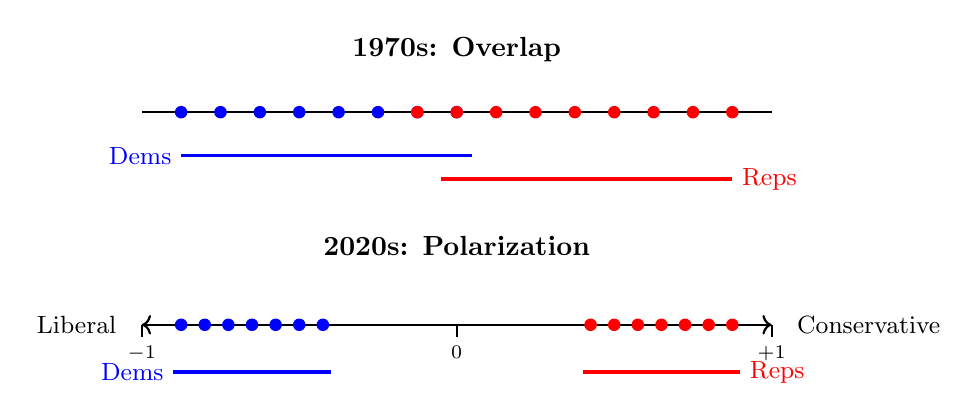
\begin{tikzpicture}[
every node/.style={font=\small},
demdot/.style={circle, fill=blue, inner sep=1.6pt},
repdot/.style={circle, fill=red, inner sep=1.6pt}
]


\node[font=\bfseries] at (0, 3.0) {1970s: Overlap};

\draw[thick] (-4, 2.2) -- (4, 2.2);


\foreach \x in {-3.5, -3.0, -2.5, -2.0, -1.5, -1.0, -0.5, 0} {
\node[demdot] at (\x, 2.2) {};
}


\foreach \x in {-0.5, 0, 0.5, 1.0, 1.5, 2.0, 2.5, 3.0, 3.5} {
\node[repdot] at (\x, 2.2) {};
}


\draw[blue, very thick] (-3.5, 1.65) -- (0.2, 1.65);
\node[blue, left, font=\small] at (-3.5, 1.65) {Dems};

\draw[red, very thick] (-0.2, 1.35) -- (3.5, 1.35);
\node[red, right, font=\small] at (3.5, 1.35) {Reps};


\node[font=\bfseries] at (0, 0.5) {2020s: Polarization};


\draw[thick, <->] (-4, -0.5) -- (4, -0.5);


\node[left, font=\small] at (-4.2, -0.5) {Liberal};
\node[right, font=\small] at (4.2, -0.5) {Conservative};


\draw[thick] (-4, -0.5) -- (-4, -0.65);
\node[below, font=\scriptsize] at (-4, -0.65) {$-1$};

\draw[thick] (0, -0.5) -- (0, -0.65);
\node[below, font=\scriptsize] at (0, -0.65) {0};

\draw[thick] (4, -0.5) -- (4, -0.65);
\node[below, font=\scriptsize] at (4, -0.65) {$+1$};

\foreach \x in {-3.5, -3.2, -2.9, -2.6, -2.3, -2.0, -1.7} {
\node[demdot] at (\x, -0.5) {};
}

\foreach \x in {1.7, 2.0, 2.3, 2.6, 2.9, 3.2, 3.5} {
\node[repdot] at (\x, -0.5) {};
}


\draw[blue, very thick] (-3.6, -1.1) -- (-1.6, -1.1);
\node[blue, left, font=\small] at (-3.6, -1.1) {Dems};

\draw[red, very thick] (1.6, -1.1) -- (3.6, -1.1);
\node[red, right, font=\small] at (3.6, -1.1) {Reps};

\end{tikzpicture}

 \framebreak
\textbf{Pattern:}
\begin{itemize}
\item 1970s: Significant overlap between parties
\item 2020s: Complete separation, no overlap
\item \alert{Polarization has increased dramatically}
\end{itemize}

We'll discuss what this means for MVT later!
\end{frame}

\begin{frame}[allowframebreaks]{Evidence 2: Trade Policy - Dutt \& Mitra (2002)}
\textbf{Question:} Does median voter's industry predict trade policy?



\textbf{Theory:}
\begin{itemize}
\item Workers in import-competing industries prefer \alert{protection} (tariffs)
\item Workers in export industries prefer \alert{free trade}
\item Median voter's industry determines policy
\end{itemize}



\textbf{Data:}
\begin{itemize}
\item Cross-country panel data
\item Industry employment shares
\item Trade protection measures (tariffs, non-tariff barriers)
\end{itemize}

 \framebreak   

\textbf{Finding:}
\begin{itemize}
\item Countries where median worker is in import-competing sector have \alert{higher protection}
\item Countries where median worker is in export sector have \alert{lower protection}
\item \alert{Consistent with median voter theorem!}
\end{itemize}
\end{frame}

\begin{frame}[allowframebreaks]{Evidence 3: Education Spending - Corcoran \& Evans (2010)}
\textbf{Question:} How does inequality affect local public spending?



\textbf{MVT prediction:}
\begin{itemize}
\item Higher inequality → median voter pays lower tax share
\item → Median voter demands more public spending
\item (They get the benefits but pay less of the cost)
\end{itemize}



\textbf{Data:}
\begin{itemize}
\item US school districts
\item Inequality measures (income distribution)
\item Education spending per pupil
\end{itemize}


  \framebreak  
\textbf{Finding:}
\begin{itemize}
\item \alert{"Results consistent with median voter model"}
\item Inequality that reduces median voter's tax share → higher local spending on education
\item Growing wealth at top lowers median voter's tax burden → they vote for more services
\end{itemize}
\end{frame}

\begin{frame}{Inequality and Education Spending: The Mechanism}
\textbf{Numerical example:}


\textbf{Low inequality scenario:}
\begin{itemize}
\item Median income = \$45k, Mean income = \$50k
\item Median voter's tax share = $45/50 = 90\%$ of average
\end{itemize}



\textbf{High inequality scenario:}
\begin{itemize}
\item Median income = \$40k, Mean income = \$70k (top-heavy distribution)
\item Median voter's tax share = $40/70 = 57\%$ of average
\end{itemize}



\textbf{Result:}
\begin{itemize}
\item In high inequality scenario, median voter gets schools funded by others
\item They pay 57\% but get 100\% of benefit
\item \alert{Incentive to vote for higher spending}
\end{itemize}



This is exactly what Corcoran \& Evans find in the data!
\end{frame}

\begin{frame}{Evidence 4: Female Suffrage - Introduction}
\textbf{Natural experiment: Expansion of voting rights to women}



\textbf{MVT prediction:}
\begin{itemize}
\item When women get the vote, median voter changes
\item If women have different preferences than men on some issues...
\item ...we should see policy changes in those areas
\end{itemize}



\textbf{Historical context:}
\begin{itemize}
\item US: Women's suffrage varied by state (1869-1920)
\item Provides variation in timing across states
\item Can use difference-in-differences methodology
\end{itemize}



\textbf{Two major studies:}
\begin{enumerate}
\item Kose et al (2021): Education outcomes
\item Miller (2008): Public health spending
\end{enumerate}
\end{frame}

\begin{frame}[allowframebreaks]{Evidence 5: Female Suffrage - Kose et al (2021)}
\textbf{Question:} Did female suffrage improve educational outcomes?



\textbf{Why might it?}
\begin{quote}
"Women's organizations in the early 20th century lobbied for the passage of children's codes to regulate child work, guardianship, and mandatory school attendance."
\end{quote}



\textbf{Data:}
\begin{itemize}
\item Variation in suffrage adoption across US states
\item Educational attainment by cohort and state
\item Focus on disadvantaged children (black children, Southern white children)
\end{itemize}


\framebreak
\textbf{Finding:}
\begin{itemize}
\item Full exposure to suffrage (ages 0-15) → \alert{+1 year of education} for black children
\item Also large effects for white children from the South
\item \alert{Consistent with median voter shifting toward pro-education policies}
\end{itemize}
\end{frame}

\begin{frame}{Evidence 6: Female Suffrage - Miller (2008)}
\textbf{Question:} Did suffrage increase public health spending?



\textbf{Theory:}
\begin{itemize}
\item Women disproportionately concerned with maternal and child health
\item Suffrage shifts median voter preferences
\item → Increased spending on public health programs
\end{itemize}



\textbf{Finding:}
\begin{itemize}
\item States that granted women's suffrage saw \alert{significant increases} in public health spending
\item Particularly on maternal and child health programs
\item Effects consistent with median voter model
\end{itemize}



\alert{Interpretation:}
\begin{itemize}
\item Politicians respond to changes in the electorate
\item When median voter shifts (due to suffrage), policy follows
\item This is exactly what MVT predicts!
\end{itemize}
\end{frame}

\begin{frame}[allowframebreaks]{Evidence 7: Local Public Goods Provision}
\textbf{Other studies finding MVT support:}



\textbf{Besley \& Case (various papers):}
\begin{itemize}
\item Gubernatorial term limits
\item When governor is term-limited, behaviour changes
\item Less responsive to median voter (no re-election incentive)
\item Evidence that electoral incentives matter
\end{itemize}



\textbf{Levitt \& Snyder (1997):}
\begin{itemize}
\item Congressional spending patterns
\item Do representatives bring federal spending to their districts?
\item Find evidence consistent with serving constituent (median voter) interests
\end{itemize}

 \framebreak   

\textbf{Common theme:}
\begin{itemize}
\item When electoral connection is strong → policies match median voter
\item When electoral connection is weak → deviation from median voter
\item \alert{Supports core MVT logic}
\end{itemize}
\end{frame}

\begin{frame}{Evidence 8: Cross-Country Social Spending}
\textbf{Broad patterns in OECD countries:}



\textbf{Correlation with median voter income:}
\begin{itemize}
\item Countries where median voter is poorer relative to mean
\item → More social spending as \% of GDP
\item → More progressive taxation
\end{itemize}



\textbf{Age structure effects:}
\begin{itemize}
\item Countries with older median voter
\item → More pension spending
\item → More healthcare spending
\end{itemize}



\textbf{Caveats:}
\begin{itemize}
\item Correlation doesn't prove causation
\item Many other factors differ across countries
\item Institutions, culture, history matter
\item But patterns are \alert{consistent with MVT}
\end{itemize}
\end{frame}

\begin{frame}{Section Summary: Evidence FOR MVT}
\textbf{What the evidence shows:}

\begin{enumerate}
\item \textbf{US politics largely one-dimensional}
\begin{itemize}
\item Poole \& Daniels: 80-90\% of votes explained by liberal-conservative spectrum
\end{itemize}


\item \textbf{Policy responds to median voter characteristics}
\begin{itemize}
\item Trade policy: Median worker's industry
\item Education spending: Median voter's tax share
\item Social spending: Median income relative to mean
\end{itemize}


\item \textbf{Suffrage expansion changed policies}
\begin{itemize}
\item Women's suffrage → education and health spending up
\item Consistent with median voter shifting
\end{itemize}


\item \textbf{Strongest support in specific settings}
\begin{itemize}
\item Single-issue votes
\item Local public goods
\item When preferences plausibly single-peaked
\end{itemize}
\end{enumerate}



\alert{But:} There's also substantial evidence that challenges MVT. Let's examine that next...
\end{frame}


\section{Empirical Challenges to MVT}

\begin{frame}{Evidence Against: Overview}
\textbf{Scientific method requires examining contradictory evidence!}


If MVT is wrong or incomplete, we should find:
\begin{itemize}
\item Identity of policymaker matters (not just constituency)
\item Party affiliation predicts votes even with identical constituencies
\item Policy doesn't respond to median voter shifts
\end{itemize}




\textbf{Three main sources of evidence:}
\begin{enumerate}
\item Randomized gender quotas in India
\item US Senate: Same state, different parties
\item US House: Close elections with identical constituencies
\end{enumerate}




\alert{Spoiler:} All three challenge MVT in important ways!
\end{frame}

\begin{frame}{Challenge 1: Indian Village Study - Setup}
\textbf{Chattopadhyay \& Duflo (2004):}


\textbf{Context:}
\begin{itemize}
\item India: 1993 constitutional amendment
\item Randomly selected villages required to reserve chief position for women
\item 1/3 of village councils (Gram Panchayats) reserved for women
\end{itemize}



\textbf{Research design:}
\begin{itemize}
\item Compare villages with female-reserved positions to control villages
\item Random assignment → no pre-treatment differences
\item \alert{Perfect natural experiment!}
\end{itemize}



\textbf{MVT prediction:}
\begin{itemize}
\item Gender of leader shouldn't matter
\item Both male and female leaders represent same constituency
\item → Same median voter → same policies
\end{itemize}
\end{frame}

\begin{frame}[allowframebreaks]{Challenge 1: Indian Village Study - Results}
\textbf{Finding:} \alert{Leaders invest more in infrastructure directly relevant to their own gender's needs}

  


\begin{center}
\includegraphics[width=0.95\textwidth]{india_villages_results.png}
\end{center}



\framebreak


\textbf{Implication:}
\begin{itemize}
\item \alert{Identity of leader matters}, not just constituency preferences
\item Same constituency, different leader → different outcomes
\item Contradicts MVT prediction
\end{itemize}
\end{frame}

\begin{frame}{Challenge 1: Interpretation}
\textbf{Why does this challenge MVT?}



\textbf{Possible explanations:}
\begin{enumerate}
\item \textbf{Information asymmetry}
\begin{itemize}
\item Female leaders better informed about women's needs
\item Know which problems are most severe
\end{itemize}


\item \textbf{Preference aggregation}
\begin{itemize}
\item Multiple issues, no clear single dimension
\item Leader's identity determines which issues get prioritized
\end{itemize}


\item \textbf{Descriptive vs. substantive representation}
\begin{itemize}
\item Having representatives "like you" matters
\item Not just about median voter's policy preference
\item Identity politics is real
\end{itemize}
\end{enumerate}



\alert{Key insight:} In multidimensional policy space, leader's identity breaks ties and determines agenda. MVT is incomplete.
\end{frame}

\begin{frame}{Challenge 2: US Senate - Setup}
\textbf{Poole \& Rosenthal (1996):}


\textbf{Observation:}
\begin{itemize}
\item Each US state has 2 senators
\item Both represent \alert{exactly the same constituency}
\item Same median voter!
\end{itemize}



\textbf{MVT prediction:}
\begin{itemize}
\item Both senators should adopt same positions
\item Should vote identically in the Senate
\item Median voter determines both senators' behaviour
\end{itemize}



\textbf{Reality:}
\begin{itemize}
\item When a state has 1 Democratic senator and 1 Republican senator...
\item ...those 2 senators vote \alert{very differently} in the Senate
\item Party affiliation trumps constituency
\end{itemize}



\alert{This directly contradicts MVT!}
\end{frame}

\begin{frame}{Challenge 2: US Senate - Evidence}
\textbf{Pattern in the data:}


\begin{itemize}
\item Compare DW-NOMINATE scores of senators from same state
\item Democratic senator: Typically -0.4 to -0.6 (liberal)
\item Republican senator: Typically +0.4 to +0.6 (conservative)
\item \alert{Enormous gap!}
\end{itemize}



\textbf{Examples:}
\begin{itemize}
\item Pennsylvania: Bob Casey (D) vs. Pat Toomey (R) - very different
\item Ohio: Sherrod Brown (D) vs. J.D. Vance (R) - opposite ends
\item Nevada: Catherine Cortez Masto (D) vs. Jacky Rosen (D) - similar!
\end{itemize}



\textbf{Interpretation:}
\begin{itemize}
\item \alert{Party matters more than constituency}
\item Senators vote with their party, not median voter
\item Party discipline, career incentives, ideology all matter
\end{itemize}
\end{frame}

\begin{frame}[allowframebreaks]{Challenge 3: US House Close Elections - Setup}
\textbf{Lee, Moretti, Butler (2004) QJE:}


\textbf{Research design:} Regression Discontinuity (RD)
\begin{itemize}
\item Compare districts where Democrat won 50.1\% vs. Republican won 50.1\%
\item Constituencies are \alert{virtually identical}
\item Only difference: party of winner
\end{itemize}



\textbf{MVT prediction:}
\begin{itemize}
\item Median voter is same in both cases
\item Democrats and Republicans elected from identical constituencies should vote similarly
\item Party shouldn't matter when median voter is the same
\end{itemize}

\framebreak

\textbf{Measurement:}
\begin{itemize}
\item ADA (Americans for Democratic Action) scores
\item 0 = most conservative, 100 = most liberal
\item Based on voting record in Congress
\end{itemize}
\end{frame}

\begin{frame}[allowframebreaks]{Challenge 3: US House Close Elections - Results}
\textbf{Finding:} \alert{Huge discontinuity at 50\% threshold}



\begin{center}
\includegraphics[width=1\textwidth]{house_discontinuity.png}
\end{center}


\framebreak


\textbf{Interpretation:}
\begin{itemize}
\item Even with \alert{identical constituencies}, party matters enormously
\item ADA scores differ by 60-80 points
\item \alert{Party identity $>$ Median voter preferences}
\end{itemize}
\end{frame}

\begin{frame}{Challenge 4: European Parliament Evidence}
\textbf{Beyond the US - similar patterns in Europe:}



\textbf{Setup:}
\begin{itemize}
\item Members of European Parliament (MEPs) from same country
\item Same national constituency
\item Different parties (left vs. right, pro-EU vs. euroskeptic)
\end{itemize}



\textbf{Finding:}
\begin{itemize}
\item MEPs vote with their \alert{party group} (EPP, S\&D, etc.)
\item Not with their national delegation
\item Party discipline is strong
\end{itemize}



\textbf{Example:}
\begin{itemize}
\item French EPP MEPs vote with German EPP MEPs
\item Not with French Socialist MEPs
\item \alert{Party $>$ Country $>$ Median voter}
\end{itemize}
\end{frame}

\begin{frame}{Party Discipline vs. Constituency Preferences}
\textbf{Why does party matter so much?}



\textbf{Institutional features:}
\begin{enumerate}
\item \textbf{Whip systems}
\begin{itemize}
\item Party leaders enforce voting discipline
\item Punishments for deviating (committee assignments, etc.)
\end{itemize}


\item \textbf{Career concerns}
\begin{itemize}
\item Advancement within party depends on loyalty
\item Party controls endorsements, funding for re-election
\end{itemize}


\item \textbf{Primary elections}
\begin{itemize}
\item Party activists (not median voter) choose nominees
\item Median primary voter $\neq$ median general election voter
\item Incentive to appeal to base, not center
\end{itemize}


\item \textbf{Ideological selection}
\begin{itemize}
\item People who become Democrats/Republicans already ideological
\item Not randomly assigned to parties
\end{itemize}
\end{enumerate}
\end{frame}

\begin{frame}{Reconciling the Evidence}
\textbf{When does MVT work? When doesn't it?}

\vspace{0.2cm}
\begin{columns}
\begin{column}{0.48\textwidth}
\textbf{MVT Works Better When:}
\begin{itemize}
\item Single, clear issue
\item Local elections
\item Weak parties
\item Direct democracy (referendums)
\item Strong electoral connection
\end{itemize}
\end{column}


\begin{column}{0.48\textwidth}
\textbf{MVT Works Worse When:}
\begin{itemize}
\item Multiple dimensions
\item Strong party discipline
\item Primary elections matter
\item National elections
\item Ideological selection
\end{itemize}
\end{column}
\end{columns}



\textbf{Bottom line:}
\begin{itemize}
\item MVT captures important forces (electoral incentives)
\item But it's \alert{incomplete} - institutions, parties, and identity matter too
\item Use MVT as baseline, then adjust for institutional details
\end{itemize}
\end{frame}

\begin{frame}{Section Summary: Evidence AGAINST MVT}
\textbf{What we've learned:}

\begin{enumerate}
\item \textbf{Identity matters}
\begin{itemize}
\item Gender of leader affects policy (India study)
\item Descriptive representation has substantive effects
\end{itemize}


\item \textbf{Party matters}
\begin{itemize}
\item Same-state senators vote differently by party
\item Close elections: party creates huge discontinuity
\item European Parliament: party groups $>$ national delegations
\end{itemize}


\item \textbf{Institutions matter}
\begin{itemize}
\item Party discipline shapes behaviour
\item Primary elections create different incentives
\item Career concerns within party
\end{itemize}


\item \textbf{MVT is not useless, but incomplete}
\begin{itemize}
\item Good in some settings (local, single-issue)
\item Limited in others (partisan, multidimensional)
\item Need richer models incorporating parties and institutions
\end{itemize}
\end{enumerate}
\end{frame}


\section{Contemporary Challenges to MVT}

\begin{frame}{The Puzzle of Modern Politics}
\href{https://www.ft.com/content/7ab73ad8-21ec-39f3-ab8d-a559a110d210}{\alert{\textbf{Diane Coyle (2015):} "Has the median voter lost her power?"}}


\begin{quote}
"Why does the mainstream middle of the political spectrum appear to have been hollowed out, with extreme parties in many countries doing well in opinion polls (if not yet elections), and the greater polarisation of major parties?"
\end{quote}



\textbf{The paradox:}
\begin{itemize}
\item MVT predicts centrist convergence
\item But we observe polarization and extremism
\item What happened?
\end{itemize}



\begin{quote}
"For many years this seemed a reasonably good account of politics in many democracies, despite being so simplistic... So what has changed recently? Why has the median voter lost her former power?"
\end{quote}
\end{frame}

\begin{frame}[allowframebreaks]{US Polarization: The Long View}
\textbf{Evidence from DW-NOMINATE scores (1880-present):}
\textbf{Historical pattern:}
\begin{itemize}
\item 1880-1900: High polarization
\item 1900-1970: Gradual convergence
\item 1970-1980: Minimal polarization (peak MVT era!)
\item 1980-present: \alert{Dramatic increase in polarization}
\end{itemize}


\textbf{Current state (2020s):}
\begin{itemize}
\item Almost \alert{no overlap} between parties in Congress
\item Most liberal Republican $>$ most conservative Democrat
\item Polarization at highest level since Civil War era
\end{itemize}

\framebreak
\begin{center}
\includegraphics[width=1.1\textwidth]{polarization_comparison.png}
\end{center}




\alert{Key question:} Is this asymmetric polarization (Republicans moving right) or symmetric (both moving)?
\begin{itemize}
\item Evidence suggests \alert{asymmetric} - Republicans moved more
\end{itemize}
\end{frame}

\begin{frame}[allowframebreaks]{The Hollowed Center}
\textbf{Two possible explanations:}
 
\textbf{Explanation 1: Voters polarized}
\begin{itemize}
\item Distribution of voter preferences has changed
\item Fewer moderate voters, more extremes
\item Bimodal distribution replaces normal distribution
\item Parties follow voters to extremes
\end{itemize}



\textbf{Explanation 2: Parties polarized (voters unchanged)}
\begin{itemize}
\item Voter preferences relatively stable
\item But parties moved for other reasons
\item Voters sort into parties after parties move
\item Parties lead, voters follow
\end{itemize}

   \framebreak 

\textbf{Evidence:}
\begin{itemize}
\item Some voter polarization (especially on cultural issues)
\item But \alert{elite polarization came first}
\item Mass polarization is partly a response to elite polarization
\end{itemize}
\end{frame}

\begin{frame}[allowframebreaks]{Possible Explanation 1: Less Rational Voters?}
\textbf{Have voters become more emotional, less rational?}



\textbf{Evidence for this view:}
\begin{itemize}
\item Rise of tribal identity politics
\item Voters seem to vote against their economic interests
\item Anger and resentment drive choices
\item "Politics as team sport"
\end{itemize}



\textbf{But:}
\begin{itemize}
\item Were voters ever purely rational?
\item Emotion always mattered in politics
\item Identity always shaped voting
\item \alert{Why would irrationality increase now?}
\end{itemize}

 \framebreak   

\textbf{Need structural explanation:}
\begin{itemize}
\item What changed in the environment?
\item What made emotional voting more salient?
\item Enter: social media...
\end{itemize}
\end{frame}

\begin{frame}[allowframebreaks]{Social Media and Information Fragmentation}
\textbf{How social media changed politics:}


\begin{enumerate}
\item \textbf{Echo chambers}
\begin{itemize}
\item Algorithms show you content you already agree with
\item Filter bubbles reduce exposure to opposing views
\item Reinforces existing beliefs
\end{itemize}


\item \textbf{Personalized news feeds}
\begin{itemize}
\item No more shared information environment
\item Different voters see different "facts"
\item Hard to find common ground
\end{itemize}

\framebreak

\item \textbf{Outrage amplification}
\begin{itemize}
\item Extreme content gets more engagement
\item Moderate voices drowned out
\item Incentive for politicians to be provocative
\end{itemize}


\item \textbf{Direct communication}
\begin{itemize}
\item Politicians bypass media gatekeepers
\item Can appeal directly to base
\item Less need to court median voter
\end{itemize}
\end{enumerate}



\alert{Result:} Harder to maintain centrist coalition when voters inhabit different information universes.
\end{frame}

\begin{frame}{Primary Elections vs. General Electorate}

\begin{center}
\includegraphics[width=0.85\textwidth]{primary_vs_general.png}
\end{center}



\textbf{The Problem:}
\begin{itemize}
\item Primary voters are more ideological than general electorate
\item Candidates optimize for primary, not general median
\item Electoral incentives pull toward base, not center
\end{itemize}
\end{frame}

\begin{frame}[allowframebreaks]{Possible Explanation 2: Return of Ideology}
\textbf{Activists and donors matter more than ever:}



\textbf{Primary electorate $\neq$ General electorate}
\begin{itemize}
\item Primary voters are more ideological
\item More engaged, more extreme
\item Median primary voter $\neq$ median general election voter
\end{itemize}



\textbf{Donor influence:}
\begin{itemize}
\item Campaign finance increasingly important
\item Donors tend to be more ideological than median voter
\item Small donors especially ideological (both left and right)
\item Candidates optimize for donors, not just voters
\end{itemize}

   \framebreak 

\textbf{Party activists:}
\begin{itemize}
\item Control nominations, endorsements
\item Punish "RINOs" (Republicans In Name Only) and moderate Democrats
\item Push candidates away from center
\end{itemize}



\alert{Result:} Electoral incentives now pull candidates toward base, not median voter.
\end{frame}

\begin{frame}{Possible Explanation 3: Multidimensional Preferences}
\textbf{Politics is no longer just left-right:}



\textbf{Multiple cleavages:}
\begin{itemize}
\item Economic redistribution (traditional left-right)
\item Cultural values (liberal-conservative)
\item Immigration (open-closed)
\item EU/Globalization (integrate-protect)
\item Climate change (action-skepticism)
\end{itemize}



\textbf{Problem for MVT:}
\begin{itemize}
\item In 5-dimensional space, \alert{no stable median}
\item No clear "center" to converge to
\item Different voters prioritize different dimensions
\item Coalition-building becomes complex
\end{itemize}



\begin{quote}
"If voters are choosing over several criteria... then there might be no stable voting outcome." - Diane Coyle
\end{quote}
\end{frame}



\begin{frame}[allowframebreaks]{Case Study: Brexit}
\textbf{Brexit didn't fit traditional left-right dimension:}



\textbf{Cross-cutting cleavages:}
\begin{itemize}
\item Traditional Labour voters (working class) voted Leave
\item Wealthy, educated Conservatives voted Remain
\item Cut across party lines
\end{itemize}



\textbf{Predictors of Leave vote:}
\begin{itemize}
\item Age (older → Leave)
\item Education (less educated → Leave)
\item Urban vs. rural (rural → Leave)
\item Immigration attitudes
\item \alert{NOT traditional left-right economic position}
\end{itemize}

  \framebreak  

\textbf{Implication:}
\begin{itemize}
\item New dimension of politics (open vs. closed)
\item Realigns voters across traditional parties
\item No clear median on this dimension initially
\end{itemize}
\end{frame}

\begin{frame}[allowframebreaks]{Case Study: US Elections 2016/2024}
\textbf{Trump's strategy: 2-dimensional positioning}



\textbf{Economic dimension:}
\begin{itemize}
\item Relatively moderate (protect Social Security, Medicare)
\item Not traditional Republican position (usually favour cuts)
\item Appeals to working-class voters
\end{itemize}



\textbf{Cultural/Identity dimension:}
\begin{itemize}
\item Extreme: immigration restrictionism, nationalism
\item "Build the wall," "Muslim ban," etc.
\item Very far from median on this dimension
\end{itemize}


  \framebreak  
\textbf{Result:}
\begin{itemize}
\item Won white working-class voters (economic moderates, cultural conservatives)
\item Lost college-educated suburbanites (economic conservatives, cultural moderates)
\item \alert{Realignment along cultural rather than economic lines}
\item Not traditional MVT convergence!
\end{itemize}
\end{frame}

\begin{frame}{Populism and Anti-Establishment Politics}
\textbf{New dimension: Elite vs. People}



\textbf{Populist framing:}
\begin{itemize}
\item "Corrupt elites" vs. "ordinary people"
\item Not about policy positions per se
\item About identity and belonging
\item "Who is politics for?"
\end{itemize}



\textbf{Examples globally:}
\begin{itemize}
\item Trump (US), Le Pen (France), Five Star (Italy)
\item Podemos (Spain), AfD (Germany)
\item Cut across traditional left-right spectrum
\end{itemize}



\textbf{MVT assumption violation:}
\begin{itemize}
\item MVT assumes policy space
\item But populism is about \alert{identity space}
\item "Are you with the people or the elite?"
\item This doesn't map onto left-right dimension
\item \alert{MVT framework struggles to explain this}
\end{itemize}
\end{frame}

\begin{frame}{Section Summary: Contemporary Challenges}
\textbf{Why has the median voter "lost power"?}


\begin{enumerate}
\item \textbf{Social media and information fragmentation}
\begin{itemize}
\item Echo chambers, filter bubbles
\item No shared information environment
\item Harder to build centrist coalitions
\end{itemize}


\item \textbf{Primary elections and activist influence}
\begin{itemize}
\item Median primary voter $\neq$ median general voter
\item Donors and activists pull parties to extremes
\end{itemize}


\item \textbf{Multidimensional politics}
\begin{itemize}
\item No longer just left-right
\item Cultural, identity, globalization dimensions
\item No clear median in multidimensional space
\end{itemize}


\item \textbf{Populism and anti-establishment}
\begin{itemize}
\item Elite vs. people framing
\item Identity politics rather than policy
\end{itemize}
\end{enumerate}



\alert{Bottom line:} MVT still captures important forces, but contemporary politics increasingly violates its assumptions!
\end{frame}


\section{Political Selection: Who Becomes a Politician?}

\begin{frame}{Transition: Selection Into Politics}
\textbf{MVT assumes politicians want to win, but...}


\begin{center}
\Large \alert{Who chooses to become a politician in the first place?}
\end{center}




\textbf{Why this matters:}
\begin{itemize}
\item If only ideologues run, MVT predictions may fail
\item If competent people avoid politics, quality of governance suffers
\item Selection affects how democracy works
\end{itemize}




\textbf{Economic theory predictions:}
\begin{itemize}
\item \alert{Adverse selection:} Lower opportunity cost → more likely to run
\item Less competent people have lower private sector earnings
\item → Politics attracts the less competent?
\end{itemize}



But is this true? Let's look at evidence from Sweden...
\end{frame}

\begin{frame}{Dal Bó et al (2017): "Who Becomes a Politician?"}
\textbf{Research question:}

\begin{quote}
"Can a democracy attract competent leaders, while attaining broad representation?"
\end{quote}



\textbf{Data:}
\begin{itemize}
\item Universe of municipal politicians in Sweden
\item Link to military conscription records (IQ, leadership tests)
\item Link to tax records (income, family background)
\item Compare politicians to general population
\end{itemize}



\textbf{Why Sweden?}
\begin{itemize}
\item Extraordinary data quality
\item Universal male conscription → IQ and leadership scores for everyone
\item Administrative data on income and background
\item Large number of municipal politicians (diverse sample)
\end{itemize}
\end{frame}

\begin{frame}{Dal Bó et al: Four Main Findings}
\textbf{Summary of results:}


\begin{enumerate}
\item \textbf{Politicians are smarter and better leaders than average}
\begin{itemize}
\item Significantly higher IQ scores
\item Higher leadership ability scores
\item \alert{Contradicts adverse selection prediction!}
\end{itemize}


\item \textbf{Representation by social background is remarkably even}
\begin{itemize}
\item Politicians come from all parts of income distribution
\item No elite capture
\end{itemize}


\item \textbf{Weak trade-off between competence and representation}
\begin{itemize}
\item High competence AND broad representation
\item Not choosing between elite competence vs. mass representation
\end{itemize}


\item \textbf{Material and intrinsic motives both matter}
\begin{itemize}
\item Higher salaries attract more competent candidates
\item But ideology and public service also drive entry
\item Party screening is important
\end{itemize}
\end{enumerate}
\end{frame}

\begin{frame}[allowframebreaks]{Finding 1: Politicians Are More Competent}
\textbf{IQ and Leadership Scores:}


\begin{itemize}
\item \alert{Cognitive ability (IQ):} Politicians score significantly higher than general population
\item \alert{Leadership ability:} Even larger difference
\item Pattern holds across all parties
\item Stronger at higher levels of government
\end{itemize}



\textbf{Why is this surprising?}
\begin{itemize}
\item Economic theory: Lower opportunity cost → more likely to enter politics
\item High-ability people earn more in private sector
\item Should see negative selection on ability
\item \alert{But we see positive selection!}
\end{itemize}

\framebreak

\textbf{Implications:}
\begin{itemize}
\item Politics attracts talent
\item Democratic institutions can select competent leaders
\item Screening mechanisms (parties, voters) work
\end{itemize}
\end{frame}

\begin{frame}{Finding 2: Broad Social Representation}
\textbf{Income and family background:}


\begin{itemize}
\item Politicians come from all parts of earnings distribution
\item No overrepresentation of economic elite
\item Remarkably even across social classes
\end{itemize}



\textbf{Why is this notable?}
\begin{itemize}
\item Common criticism: Politics is for the rich
\item Elite capture of political institutions
\item \alert{Sweden shows it's possible to have broad representation}
\end{itemize}



\textbf{Mechanisms in Sweden:}
\begin{itemize}
\item PR system (easier for working-class candidates to get elected)
\item Strong party organizations (provide support and resources)
\item Public financing of elections (reduces money barrier)
\item Union representation in left parties
\end{itemize}
\end{frame}

\begin{frame}{Finding 3: Competence and Representation - Weak Trade-Off}
\textbf{The surprising result:}


Countries often face a perceived trade-off:
\begin{itemize}
\item Elite politicians: High competence, low representation
\item Mass politicians: Low competence, high representation
\end{itemize}



\textbf{Sweden defies this:}
\begin{itemize}
\item \alert{High competence AND broad representation}
\item Selection on competence doesn't exclude working-class candidates
\item Smart people exist at all income levels
\item Parties recruit from broad base
\end{itemize}



\textbf{Implication:}
\begin{itemize}
\item Institutions matter for who enters politics
\item Well-designed systems can get both competence and representation
\item Not inevitable that we choose one or the other
\end{itemize}
\end{frame}

\begin{frame}{Finding 4: Why Do People Become Politicians?}
\textbf{Material vs. intrinsic motivation:}



\textbf{Material motives (salaries):}
\begin{itemize}
\item Higher salaries → \alert{more competent candidates} enter
\item Effect is significant and robust
\item Money matters for attracting talent
\end{itemize}



\textbf{Intrinsic motives (ideology, public service):}
\begin{itemize}
\item People care about policy outcomes
\item Civic duty and public service motivation
\item Party affiliation reflects values, not just career
\end{itemize}



\textbf{Party screening:}
\begin{itemize}
\item Parties act as gatekeepers
\item Select candidates based on competence and fit
\item Provide training and support
\item \alert{This matters for quality of political class}
\end{itemize}
\end{frame}

\begin{frame}{Selection vs. Treatment Effects}
\textbf{Important distinction:}



\textbf{Selection:} Do certain types of people become politicians?
\begin{itemize}
\item Dal Bó et al: Smart, capable people enter politics
\item Self-selection based on ability
\end{itemize}



\textbf{Treatment:} Does being a politician change you?
\begin{itemize}
\item Do politicians become more centrist after election?
\item Or do they stick to their pre-election positions?
\item Less evidence on this question
\end{itemize}



\textbf{Relevance for MVT:}
\begin{itemize}
\item If politicians are ideologically committed (selection)
\item → Less likely to converge to median voter
\item If politicians are flexible (treatment)
\item → More likely to respond to electoral incentives
\end{itemize}
\end{frame}

\begin{frame}{Career Politicians vs. Outsiders}
\textbf{Recent trend: Rise of political outsiders}



\textbf{Examples:}
\begin{itemize}
\item Trump (business background, no political experience)
\item Zelenskyy (comedian/actor → President of Ukraine)
\item Five Star Movement in Italy (anti-establishment)
\end{itemize}



\textbf{Question:} Does lack of political experience correlate with extremism?
\begin{itemize}
\item Career politicians socialized into norms
\item Understand need for compromise
\item Outsiders less constrained by party
\item May take more extreme positions
\end{itemize}



\textbf{Evidence:} Mixed
\begin{itemize}
\item Some outsiders are moderate pragmatists
\item Others are ideological extremists
\item Depends on why they entered politics
\end{itemize}
\end{frame}

\begin{frame}{Does Competence Correlate with Centrism?}
\textbf{Open question:}


\begin{itemize}
\item Dal Bó et al: Politicians are more competent than average
\item \alert{But:} Are more competent politicians also more moderate?
\end{itemize}



\textbf{Possible mechanisms:}
\begin{itemize}
\item Smart people understand trade-offs and complexity
\item → More likely to be moderate?
\item Or: Smart people better at justifying extreme positions
\item → No relationship?
\end{itemize}



\textbf{Limited evidence:}
\begin{itemize}
\item Some studies find educated elites are more extreme
\item Others find competence correlates with pragmatism
\item \alert{Needs more research}
\end{itemize}
\end{frame}

\begin{frame}{Section Summary: Political Selection}
\textbf{What we've learned:}

\begin{enumerate}
\item \textbf{Politicians are more competent than average (Dal Bó et al)}
\begin{itemize}
\item Higher IQ and leadership ability
\item Contradicts adverse selection prediction
\end{itemize}


\item \textbf{Broad social representation is possible}
\begin{itemize}
\item Sweden achieves both competence and representation
\item Institutions matter
\end{itemize}


\item \textbf{Material and intrinsic motives both matter}
\begin{itemize}
\item Salaries attract talent
\item But ideology and public service also drive entry
\end{itemize}


\item \textbf{Selection affects MVT predictions}
\begin{itemize}
\item If politicians are ideologically committed → less convergence
\item If they're office-motivated → more convergence
\item Understanding selection helps explain deviations from MVT
\end{itemize}
\end{enumerate}
\end{frame}

\section{Normative Analysis: Should We Want Median Voter Outcomes?}

\begin{frame}{Positive vs. Normative Analysis}
\textbf{Two distinct questions:}


\begin{columns}
\begin{column}{0.48\textwidth}
\textbf{Positive (Descriptive)}
\begin{itemize}
\item \textit{Does} MVT describe reality?
\item What do we observe?
\item When does it work?
\item Scientific question
\end{itemize}
\end{column}


\begin{column}{0.48\textwidth}
\textbf{Normative (Prescriptive)}
\begin{itemize}
\item \alert{\textit{Should} we want median voter outcomes?}
\item Is it desirable?
\item Is it just?
\item Philosophical question
\end{itemize}
\end{column}
\end{columns}



\textbf{Why ask normative questions?}
\begin{itemize}
\item Understanding MVT helps us design institutions
\item Should we strengthen or weaken median voter's power?
\item What are alternatives?
\item Trade-offs between different values
\end{itemize}
\end{frame}

\begin{frame}{When Is Median Voter Outcome Desirable?}
\textbf{MVT looks good when:}


\begin{enumerate}
\item \textbf{Preferences are symmetric}
\begin{itemize}
\item Median = Mean
\item Median voter represents "average" citizen
\item Maximizing median welfare = maximizing average welfare
\end{itemize}


\item \textbf{Utilitarian welfare maximization}
\begin{itemize}
\item If we want to maximize total utility
\item And median = mean
\item Then MVT outcome is efficient
\end{itemize}


\item \textbf{Single-peaked preferences}
\begin{itemize}
\item Condorcet winner exists
\item Stable, predictable outcomes
\item Democratic legitimacy
\end{itemize}
\end{enumerate}



\textbf{But:} What if we care about rights, not just utility? What about minorities?
\end{frame}

\begin{frame}{Majority Tyranny Concerns}
\textbf{Classic warnings from political philosophy:}



\textbf{John Stuart Mill:}
\begin{quote}
"The tyranny of the majority is now generally included among the evils against which society requires to be on its guard."
\end{quote}



\textbf{Alexis de Tocqueville:}
\begin{quote}
"...a majority of the citizens are capable of oppressing the remaining minority."
\end{quote}



\textbf{The problem:}
\begin{itemize}
\item 51\% can impose on 49\%
\item Intensity of preferences ignored
\item Minorities can be systematically disadvantaged
\item What if median voter wants to violate minority rights?
\end{itemize}
\end{frame}

\begin{frame}{The Intensity Problem Returns}
\textbf{Recall from earlier: One person, one vote ignores intensity}



\textbf{Example:}
\begin{itemize}
\item 60\% mildly prefer policy A
\item 40\% passionately oppose policy A
\item Majority rule → policy A wins
\item But total utility might be higher with policy B!
\end{itemize}



\textbf{When is this most problematic?}
\begin{itemize}
\item Minority rights issues
\item Religious or cultural practices
\item Fundamental freedoms
\item Identity and dignity
\end{itemize}



\alert{Solution:} Constitutional protections, rights that can't be voted away, supermajority requirements for certain decisions.
\end{frame}

\begin{frame}[allowframebreaks]{Minority Representation}
\textbf{Two types of representation:}



\textbf{Descriptive representation:}
\begin{itemize}
\item Legislature "looks like" the population
\item Diverse by race, gender, class, etc.
\item Symbolic importance
\end{itemize}



\textbf{Substantive representation:}
\begin{itemize}
\item Policies address minority group interests
\item Not just about who is elected
\item About what policies are enacted
\end{itemize}

  \framebreak  

\textbf{MVT and minority representation:}
\begin{itemize}
\item Pure MVT: Majority always wins, minorities lose
\item Solutions:
\begin{itemize}
\item Reserved seats (like India study)
\item Proportional representation
\item Coalition governments
\item Consociational democracy
\end{itemize}
\end{itemize}
\end{frame}

\begin{frame}{Alternative Voting Systems}
\textbf{How different electoral systems relate to MVT:}


\begin{table}
\centering
\small
\begin{tabular}{lll}
\toprule
\textbf{System} & \textbf{MVT Relevance} & \textbf{Minority Rep.} \\
\midrule
FPTP (US/UK) & High & Low \\
& Two-party, convergence & Winner-take-all \\
\midrule
PR (Netherlands) & Low & High \\
& Many parties, coalitions & Proportional seats \\
\midrule
PR-STV (Ireland) & Medium & Medium \\
& Multi-seat, transfers & Better than FPTP \\
\midrule
Ranked Choice & Medium & Medium \\
& Instant runoff & Reduces spoilers \\
\bottomrule
\end{tabular}
\end{table}



\textbf{Trade-off:}
\begin{itemize}
\item FPTP → Strong MVT forces, weak minority representation
\item PR → Weak MVT forces, strong minority representation
\item No perfect system!
\end{itemize}
\end{frame}

\begin{frame}[allowframebreaks]{Irish PR-STV: A Compromise?}
\textbf{How does Ireland's system balance these concerns?}



\textbf{Features:}
\begin{itemize}
\item Proportional representation (better for minorities than FPTP)
\item Multi-seat constituencies (3-5 seats)
\item Single Transferable Vote (preference ranking)
\item Local accountability (constituency service)
\end{itemize}



\textbf{Effects:}
\begin{itemize}
\item More parties than FPTP (FF, FG, SF, Lab, Greens, others)
\item Coalition governments are norm
\item Independents can win seats
\item \alert{But:} Still majoritarian in practice (government formation)
\end{itemize}


 \framebreak   
\textbf{MVT implications:}
\begin{itemize}
\item Less pure MVT convergence than FPTP
\item But coalition formation reintroduces median voter logic
\item Need to appeal to median to form government
\end{itemize}
\end{frame}

\begin{frame}{Trade-Offs in Democratic Design}
\textbf{No perfect electoral system (Arrow's theorem again!)}


\begin{columns}
\begin{column}{0.48\textwidth}
\textbf{Representation}
\begin{itemize}
\item Minority voices heard
\item Proportional outcomes
\item Diverse legislature
\end{itemize}
\end{column}


\begin{column}{0.48\textwidth}
\textbf{Governability}
\begin{itemize}
\item Clear accountability
\item Decisive action
\item Stable government
\end{itemize}
\end{column}
\end{columns}



\begin{columns}
\begin{column}{0.48\textwidth}
\textbf{Extremism vs. Coalition Compromise}
\begin{itemize}
\item Niche parties vs. broad coalitions
\item Ideological purity vs. pragmatism
\end{itemize}
\end{column}


\begin{column}{0.48\textwidth}
\textbf{Median Voter Power}
\begin{itemize}
\item Centrist policies
\item But risk of tyranny of majority
\end{itemize}
\end{column}
\end{columns}



\alert{Different societies make different choices based on their values and history.}
\end{frame}

\begin{frame}[allowframebreaks]{Future of Majoritarian Democracy}
\textbf{Is the median voter model still relevant?}



\textbf{Challenges:}
\begin{itemize}
\item Multidimensional politics
\item Polarization
\item Social media fragmentation
\item Rise of populism
\end{itemize}



\textbf{But:}
\begin{itemize}
\item Electoral incentives still exist
\item Median voter logic applies in some contexts
\item Useful benchmark even when violated
\end{itemize}

\framebreak

\textbf{Adaptation:}
\begin{itemize}
\item More sophisticated models (multidimensional, probabilistic)
\item Incorporate parties, institutions, social media
\item Behavioral insights
\item \alert{MVT is a building block, not the complete theory}
\end{itemize}
\end{frame}


\section{Conclusion}

\begin{frame}{Applying MVT: A Decision Framework}
\textbf{When analyzing a political situation, ask:}


\begin{center}
\includegraphics[width=0.7\textwidth]{mvt_decision_tree.png}
\end{center}


Use this framework to assess whether MVT predictions will hold!
\end{frame}

\begin{frame}{Summary: When Does MVT Work Well?}
\textbf{MVT predictions are strongest when:}

\begin{enumerate}
\item \textbf{Single-dimensional issues}
\begin{itemize}
\item Tax rates, spending levels
\item Can order alternatives on a line
\end{itemize}


\item \textbf{Two-party/candidate competition}
\begin{itemize}
\item FPTP systems
\item Clear left-right competition
\end{itemize}


\item \textbf{Single-peaked preferences}
\begin{itemize}
\item Everyone has ideal point
\item Preferences decline moving away
\end{itemize}


\item \textbf{Strong electoral connection}
\begin{itemize}
\item Re-election matters
\item Weak party discipline
\item Responsive politicians
\end{itemize}


\item \textbf{Local public goods decisions}
\begin{itemize}
\item School spending, park locations
\item Simpler, more direct accountability
\end{itemize}
\end{enumerate}
\end{frame}

\begin{frame}{Summary: When Does MVT Fail?}
\textbf{MVT struggles when:}

\begin{enumerate}
\item \textbf{Multiple dimensions}
\begin{itemize}
\item Economic + cultural + identity + globalization
\item No stable equilibrium
\end{itemize}


\item \textbf{Strong party discipline}
\begin{itemize}
\item Party whips enforce voting
\item Career concerns within party
\item Party $>$ constituency
\end{itemize}


\item \textbf{Primary electorates matter}
\begin{itemize}
\item Median primary voter $\neq$ median general voter
\item Base mobilization vs. center appeal
\end{itemize}


\item \textbf{Money in politics}
\begin{itemize}
\item Donors pull candidates to extremes
\item Fundraising incentives
\end{itemize}


\item \textbf{Ideological politicians}
\begin{itemize}
\item Policy-motivated, not just office-motivated
\item Willing to lose rather than compromise
\end{itemize}
\end{enumerate}
\end{frame}

\begin{frame}{Open Research Questions}
\textbf{What we still need to understand better:}


\begin{enumerate}
\item \textbf{How many dimensions in modern politics?}
\begin{itemize}
\item Can we reduce to 2-3 dimensions?
\item Or truly 5+ dimensional?
\end{itemize}


\item \textbf{Can we measure the median voter?}
\begin{itemize}
\item In multidimensional space
\item With imperfect information
\end{itemize}


\item \textbf{Effect of polarization on governance}
\begin{itemize}
\item Does polarization harm policy quality?
\item Or is it just redistribution of power?
\end{itemize}


\item \textbf{Role of social media}
\begin{itemize}
\item Does it fundamentally change electoral incentives?
\item Or just amplify existing trends?
\end{itemize}


\item \textbf{Institutional design}
\begin{itemize}
\item What electoral systems best balance representation and governability?
\item How to protect minorities while respecting majority rule?
\end{itemize}
\end{enumerate}
\end{frame}

\begin{frame}{Final Takeaway}
\begin{center}
 \textbf{George Box (1976):}
\begin{quote}
"All models are wrong, but some are useful."
\end{quote}
\end{center}


\textbf{The Median Voter Theorem is useful because:}
\begin{itemize}
\item Provides a clear baseline prediction
\item Helps us understand when reality deviates (and why)
\item Clarifies the forces pushing toward convergence
\item Shows what's required for democratic stability
\end{itemize}




\textbf{But it's wrong in important ways:}
\begin{itemize}
\item Parties matter
\item Institutions matter
\item Identity matters
\item Multidimensionality matters
\end{itemize}




\alert{Understanding both the power and limits of MVT makes us better analysts of democratic politics!}
\end{frame}

\begin{frame}{Irish Context: Party Positioning}
\textbf{Do Irish parties converge to the median voter?}


\begin{center}
\includegraphics[width=0.9\textwidth]{irish_parties_positioning.png}
\end{center}



\textbf{Discussion questions:}
\begin{itemize}
\item Why are FF and FG so close together?
\item Is SF's left position consistent with MVT or challenging it?
\item Is the median Irish voter shifting left?
\end{itemize}
\end{frame}

\begin{frame}{Next Steps \& Assignments}
\textbf{Before next week:}
\begin{enumerate}
\item Review MVT readings (posted on Loop/GitHub)
\item Start thinking about your Irish Context presentation:
\begin{itemize}
\item Week 4: Do FF/FG/SF converge toward median Irish voter?
\item How does PR-STV change MVT predictions?
\item What about Sinn Féin's rise?
\end{itemize}
\item Begin considering Project 1 paper selection
\end{enumerate}


\textbf{Next week's topic:}
\begin{itemize}
\item Political Competition and Macroeconomic Performance
\item Do politicians manipulate the economy before elections?
\item Political business cycles
\end{itemize}
\end{frame}



\section*{Further Reading}

\begin{frame}{Foundational Works (1940s-1960s)}
\footnotesize
\begin{enumerate}
\item Wicksell, K. (1896). \emph{Finanztheoretische Untersuchungen}. ["A New Principle of Just Taxation"]
\item Black, D. (1948). "On the Rationale of Group Decision-making." \emph{Journal of Political Economy}, 56(1), 23-34.
\item Arrow, K. J. (1951). \emph{Social Choice and Individual Values}. New York: Wiley. (Nobel Prize 1972)
\item Downs, A. (1957). \emph{An Economic Theory of Democracy}. New York: Harper \& Row.
\item Buchanan, J. M., \& Tullock, G. (1962). \emph{The Calculus of Consent}. Ann Arbor: University of Michigan Press.
\item Olson, M. (1965). \emph{The Logic of Collective Action}. Cambridge, MA: Harvard University Press.
\end{enumerate}


\textbf{These are the classics} that established Public Choice and the median voter framework.
\end{frame}

\begin{frame}{Theoretical Development (1970s-1990s)}
\footnotesize
\begin{enumerate}
\setcounter{enumi}{6}
\item McKelvey, R. D. (1976). "Intransitivities in Multidimensional Voting Models." \emph{Econometrica}, 44(3), 472-487.
\item Schofield, N. (1978). "Instability of Simple Dynamic Games." \emph{Review of Economic Studies}, 45(3), 575-594.
\item Meltzer, A. H., \& Richard, S. F. (1981). "A Rational Theory of the Size of Government." \emph{Journal of Political Economy}, 89(5), 914-927.
\item Wittman, D. (1983). "Candidate Motivation: A Synthesis of Alternative Theories." \emph{American Political Science Review}, 77(1), 142-157.
\item Poole, K. T., \& Daniels, R. S. (1985). "Ideology, Party, and Voting in the US Congress." \emph{American Political Science Review}, 79(2), 373-399.
\item Poole, K. T., \& Rosenthal, H. (1996). \emph{Congress: A Political-Economic History of Roll Call Voting}. Oxford University Press.
\end{enumerate}
\end{frame}

\begin{frame}{Empirical Studies: Supporting Evidence}
\footnotesize
\begin{enumerate}
\setcounter{enumi}{12}
\item Levitt, S. D., \& Snyder, J. M. (1997). "The Impact of Federal Spending on House Election Outcomes." \emph{Journal of Political Economy}, 105(1), 30-53.
\item Dutt, P., \& Mitra, D. (2002). "Endogenous Trade Policy Through Majority Voting." \emph{Journal of International Economics}, 58(1), 107-133.
\item Miller, G. (2008). "Women's Suffrage, Political Responsiveness, and Child Survival." \emph{Quarterly Journal of Economics}, 123(3), 1287-1327.
\item Corcoran, S. P., \& Evans, W. N. (2010). "Income Inequality, the Median Voter, and Local School Expenditure." \emph{Journal of Urban Economics}, 68(2), 221-236.
\item Kose, E., Kuka, E., \& Shenhav, N. (2021). "Women's Suffrage and Children's Education." \textit{American Economic Journal: Economic Policy}, 13(3), 374--405.
\end{enumerate}
\end{frame}

\begin{frame}{Empirical Studies: Challenging Evidence}
\footnotesize
\begin{enumerate}
\setcounter{enumi}{17}
\item Chattopadhyay, R., \& Duflo, E. (2004). "Women as Policy Makers: Evidence from a Randomized Policy Experiment in India." \emph{Econometrica}, 72(5), 1409-1443.
\item Lee, D. S., Moretti, E., \& Butler, M. J. (2004). "Do Voters Affect or Elect Policies?" \emph{Quarterly Journal of Economics}, 119(3), 807-859.
\item Bertrand, M., \& Mullainathan, S. (2001). "Are CEOs Rewarded for Luck?" \emph{QJE}, 116(3), 901-932. [Cited for comparison]
\item Besley, T., \& Case, A. (1995). "Does Electoral Accountability Affect Economic Policy Choices?" \emph{QJE}, 110(3), 769-798.
\end{enumerate}
\end{frame}

\begin{frame}{Political Selection \& Contemporary Challenges}
\footnotesize
\begin{enumerate}
\setcounter{enumi}{21}
\item Dal Bó, E., Finan, F., Folke, O., Persson, T., \& Rickne, J. (2017). "Who Becomes a Politician?" \emph{Quarterly Journal of Economics}, 132(4), 1877-1914.
\item Fiorina, M. P. (2017). \emph{Unstable Majorities: Polarization, Party Sorting, and Political Stalemate}. Hoover Institution Press.
\item McCarty, N., Poole, K. T., \& Rosenthal, H. (2016). \emph{Polarized America: The Dance of Ideology and Unequal Riches} (2nd ed.). MIT Press.
\item Levendusky, M. (2009). \emph{The Partisan Sort: How Liberals Became Democrats and Conservatives Became Republicans}. University of Chicago Press.
\end{enumerate}
\end{frame}

\begin{frame}{Recent Applications \& Extensions}
\footnotesize
\begin{enumerate}
\setcounter{enumi}{25}
\item Persson, T., \& Tabellini, G. (2002). \emph{Political Economics: Explaining Economic Policy}. MIT Press.
\item Acemoglu, D., \& Robinson, J. A. (2006). \emph{Economic Origins of Dictatorship and Democracy}. Cambridge University Press.
\item Caplan, B. (2007). \emph{The Myth of the Rational Voter: Why Democracies Choose Bad Policies}. Princeton University Press.
\item Alesina, A., \& Giuliano, P. (2011). "Preferences for Redistribution." In \emph{Handbook of Social Economics}.
\item Autor, D., Dorn, D., Hanson, G., \& Majlesi, K. (2020). "Importing Political Polarization? The Electoral Consequences of Rising Trade Exposure." \emph{American Economic Review}, 110(10), 3139-3183.
\end{enumerate}
\end{frame}

\begin{frame}{Textbooks \& Surveys}
\footnotesize
\begin{enumerate}
\setcounter{enumi}{30}
\item Mueller, D. C. (2003). \emph{Public Choice III}. Cambridge University Press. [Chapter 11]
\item Persson, T., \& Tabellini, G. (2000). \emph{Political Economics: Explaining Economic Policy}. MIT Press.
\item Drazen, A. (2000). \emph{Political Economy in Macroeconomics}. Princeton University Press.
\item Congleton, R. D., Hillman, A. L., \& Konrad, K. A. (Eds.). (2008). \emph{40 Years of Research on Rent Seeking} (Vols. 1-2). Springer.
\item Ashworth, S. (2012). "Electoral Accountability: Recent Theoretical and Empirical Work." \emph{Annual Review of Political Science}, 15, 183-201.
\end{enumerate}


\textbf{Encyclopedias:}
\begin{itemize}
\item Entry on "Median Voter Theorem" in \emph{Encyclopedia of Public Choice} (Shughart \& Razzolini, 2001)
\item Entry on "Downs, Anthony" in \emph{The New Palgrave Dictionary of Economics}
\end{itemize}
\end{frame}

\begin{frame}{Online Resources \& Lectures}
\footnotesize
\textbf{MIT OpenCourseWare:}
\begin{itemize}
\item Benjamin Olken. 14.75 Political Economy and Economic Development. Fall 2012. \url{https://ocw.mit.edu}
\item Emmanuel Saez lecture notes: \url{http://eml.berkeley.edu/~saez/course131/political_ch09_new.pdf}
\end{itemize}


\textbf{Journalism \& Commentary:}
\begin{itemize}
\item Cowen, T. (2010). "In Politics, Sometimes the Middle Way Really Is the Best." \emph{New York Times}. \url{http://www.nytimes.com/2010/02/07/business/economy/07view.html}
\item Coyle, D. (2015). "Has the median voter lost her power?" \emph{Financial Times}. \url{https://www.ft.com/content/7ab73ad8-21ec-39f3-ab8d-a559a110d210}
\end{itemize}


\textbf{Data Resources:}
\begin{itemize}
\item Voteview.com (DW-NOMINATE scores for US Congress)
\item ANES (American National Election Studies)
\item European Social Survey
\end{itemize}
\end{frame}


\section*{Cultural Resources}

\begin{frame}{Films \& TV Series}
\textbf{Political Competition \& Electoral Strategy:}
\begin{itemize}
\item \textbf{The West Wing} (Season 3, Episodes on polling and positioning)
\item \textbf{The War Room} (1993 documentary) - Clinton campaign strategists
\item \textbf{Veep} - Satirical take on campaign positioning
\item \textbf{Parks and Recreation} - Local government and median voter
\item \textbf{Borgen} (Danish series) - Coalition politics in PR system
\end{itemize}


\textbf{Polarization \& Contemporary Politics:}
\begin{itemize}
\item \textbf{The Social Dilemma} (Netflix) - Social media and polarization
\item \textbf{Get Me Roger Stone} (Netflix) - Partisan strategy
\item \textbf{Brexit: The Uncivil War} (2019) - Campaign strategy
\end{itemize}
\end{frame}

\begin{frame}{Books for General Audience}
\textbf{Directly relevant to MVT:}
\begin{itemize}
\item Bryan Caplan - \emph{The Myth of the Rational Voter} (2007)
\item Morris Fiorina - \emph{Culture War? The Myth of a Polarized America} (3rd ed., 2010)
\item Ezra Klein - \emph{Why We're Polarized} (2020)
\end{itemize}


\textbf{On electoral systems:}
\begin{itemize}
\item Arend Lijphart - \emph{Patterns of Democracy} (1999)
\item David Farrell - \emph{Electoral Systems: A Comparative Introduction} (2011)
\end{itemize}


\textbf{Irish politics:}
\begin{itemize}
\item Michael Gallagher et al. - \emph{Politics in the Republic of Ireland} (6th ed., 2018)
\item Eoin O'Malley - \emph{Contemporary Ireland} (2011)
\end{itemize}
\end{frame}

\begin{frame}[allowframebreaks]{Podcasts \& Online Media}
\textbf{Political Economy Podcasts:}
\begin{itemize}
\item \textbf{EconTalk} (Russ Roberts)
\begin{itemize}
\item Morris Fiorina on polarization
\item Bryan Caplan on rational voting
\item Multiple episodes on public choice
\end{itemize}
\item \textbf{The Ezra Klein Show} - Episodes on polarization and electoral systems
\item \textbf{Planet Money} - "The Median Voter" episode
\end{itemize}

   \framebreak 
\textbf{Data Journalism:}
\begin{itemize}
\item \textbf{FiveThirtyEight Politics} - Electoral analysis and polling
\item \textbf{The Economist Asks} - Episodes on democracy and voting
\item \textbf{More or Less} (BBC Radio 4) - Statistical thinking in politics
\end{itemize}


\textbf{Irish Context:}
\begin{itemize}
\item \textbf{The Irish Politics Podcast}
\item \textbf{Oireachtas TV} - Dáil debates
\item \textbf{RTÉ Archives} - Historical election coverage
\end{itemize}
\end{frame}

\begin{frame}[allowframebreaks]{How to Engage with These Resources}
\textbf{Suggested approach for deeper learning:}

\begin{enumerate}
\item \textbf{Pick resources that interest you}
\begin{itemize}
\item Don't feel obligated to consume everything
\item Follow your curiosity
\end{itemize}

\item \textbf{Watch/read/listen with MVT in mind:}
\begin{itemize}
\item Are politicians trying to appeal to median voter?
\item What prevents convergence?
\item Which assumptions are violated?
\end{itemize}
 \framebreak   
\item \textbf{Connect to Irish context:}
\begin{itemize}
\item How would this apply in Ireland?
\item Does PR-STV change the analysis?
\item Use in your presentations!
\end{itemize}

\item \textbf{Discuss with peers:}
\begin{itemize}
\item Presentations are opportunities for debate
\item Bring in examples from these resources
\item Challenge the theories
\end{itemize}
\end{enumerate}


\alert{Remember:} Cultural resources complement academic reading but don't replace it!
\end{frame}

\begin{frame}{Final Thought}
\begin{center}
\large "Democracy is the worst form of government – except for all the others that have been tried." \\

- Winston Churchill
\end{center}



\begin{center}
The median voter theorem helps us understand \textit{why} democracy works as well as it does...


...and why it sometimes doesn't work as well as we'd hope.


\textbf{Understanding the mechanism is the first step to improving it.}
\end{center}
\end{frame}


\end{document}